\documentclass{article}


\usepackage{arxiv}

\usepackage[utf8]{inputenc} % allow utf-8 input
\usepackage[T1]{fontenc}    % use 8-bit T1 fonts
\usepackage{hyperref}       % hyperlinks
\usepackage{url}            % simple URL typesetting
\usepackage{booktabs}       % professional-quality tables
\usepackage{amsfonts}       % blackboard math symbols
\usepackage{nicefrac}       % compact symbols for 1/2, etc.
\usepackage{microtype}      % microtypography
\usepackage{lipsum}
\usepackage{graphicx}
\graphicspath{ {./images/} }
\DeclareUnicodeCharacter{200A}{!!!FIX ME!!!} 

\title{Transformer models: an introduction and catalog}

\author{
 Xavier Amatriain \\
  Los Gatos, CA 95032 \\
  \texttt{xavier@amatriain.net} \\
  %% examples of more authors
 \\
}

\begin{document}
\maketitle
\begin{abstract}
In the past few years we have seen the meteoric appearance of dozens of models of the Transformer family, all of which have funny, but not self-explanatory, names. The goal of this paper is to offer a somewhat comprehensive but simple catalog and classification of the most popular Transformer models. The paper also includes an introduction to the most important aspects and innovation in Transformer models.
\end{abstract}

\tableofcontents

% keywords can be removed
%\keywords{First keyword \and Second keyword \and More}


\section{Introduction: What are Transformers}

Transformers are a class of deep learning models that are defined by some architectural traits. They were first introduced in the now famous "Attention is All you Need" paper by Google researchers in 2017 \cite{vaswani2017attention} (the paper has accumulated a whooping 38k citations in only 5 years) and associated blog post\footnote{\url{https://ai.googleblog.com/2017/08/transformer-novel-neural-network.html}}.

The Transformer architecture is a specific instance of the encoder-decoder models\cite{cho2014properties}\footnote{https://machinelearningmastery.com/encoder-decoder-long-short-term-memory-networks/} that had become popular just over the 2–3 years prior. Up until that point however, attention was just one of the mechanisms used by these models, which were mostly based on LSTM (Long Short Term Memory)\cite{hochreiter1997long} and other RNN (Recurrent Neural Networks)\cite{mikolov2010recurrent} variations. The key insight of the Transformers paper was that, as the title implies, attention could be used as the only mechanism to derive dependencies between input and output.

It is beyond the scope of this blog to go into all the details of the Transformer architecture. For that, I will refer you to the original paper above or to the wonderful The Illustrated Transformer\footnote{\url{https://jalammar.github.io/illustrated-transformer/}} post. That being said, we will briefly describe the most important aspects since we will be referring to them in the catalog below. Let’s start with the basic architectural diagram from the original paper, and describe some of the components.



\subsection{Encoder/Decoder architecture}

A generic encoder/decoder architecture (see Figure \ref{fig:transformer}) is made up of two models. The encoder takes the input and encodes it into a fixed-length vector. The decoder takes that vector and decodes it into the output sequence. The encoder and decoder are jointly trained to minimize the conditional log-likelihood. Once trained the encoder/decoder can generate an output given an input sequence or can score a pair of input/output sequences.

\begin{figure}
    \centering
    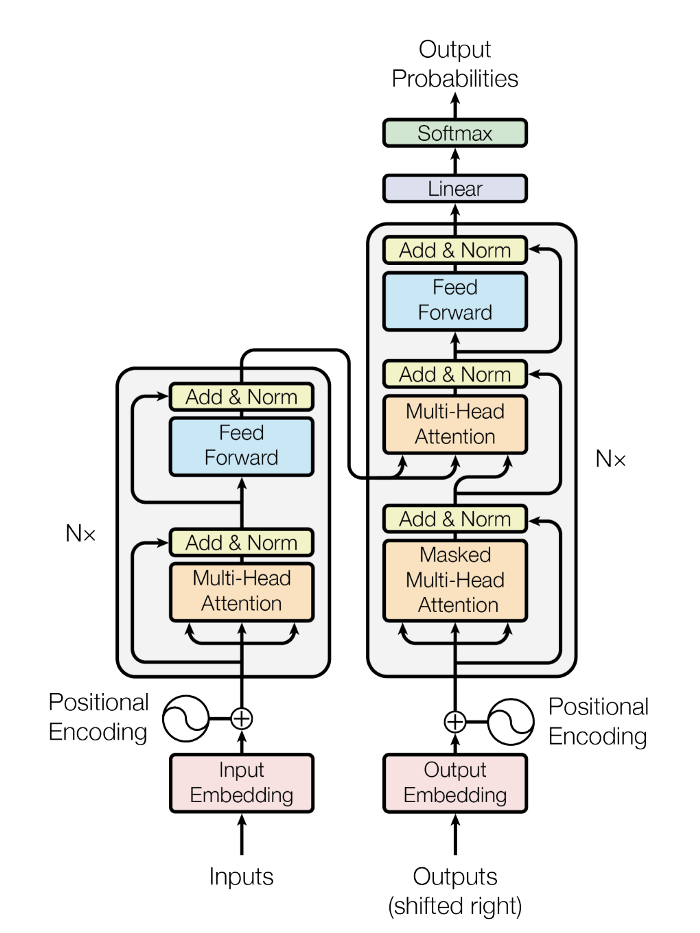
\includegraphics[width=\textwidth,height=\textheight,keepaspectratio]{02-02.png}
    \caption{Transformer Architecture from \cite{vaswani2017attention}}
    \label{fig:transformer}
\end{figure}

In the case of the original Transformer architecture, both encoder and decoder had 6 identical layers. In each of those 6 layers the Encoder has two sub layers: a multi-head attention layer, and a simple feed forward network. Each sublayer has a residual connection and a layer normalization. The output size of the Encoder is 512. The Decoder adds a third sublayer, which is another multi-head attention layer over the output of the Encoder. Besides, the other multi-head layer in the decoder is masked to prevent attention to subsequent positions.

\subsection{Attention}

It is clear from the description above that the only “exotic” elements of the model architecture are the multi-headed attention, but, as described above, that is where the whole power of the model lies! So, what is attention anyway? An attention function is a mapping between a query and a set of key-value pairs to an output. The output is computed as a weighted sum of the values, where the weight assigned to each value is computed by a compatibility function of the query with the corresponding key. Transformers use multi-headed attention, which is a parallel computation of a specific attention function called scaled dot-product attention. I will refer you again to the The Illustrated Transformer\footnote{\url{https://jalammar.github.io/illustrated-transformer/}} post for many more details on how the attention mechanism works, but will reproduce the diagram from the original paper in Figure \ref{fig:attention} so you get the main idea

\begin{figure}
    \centering
    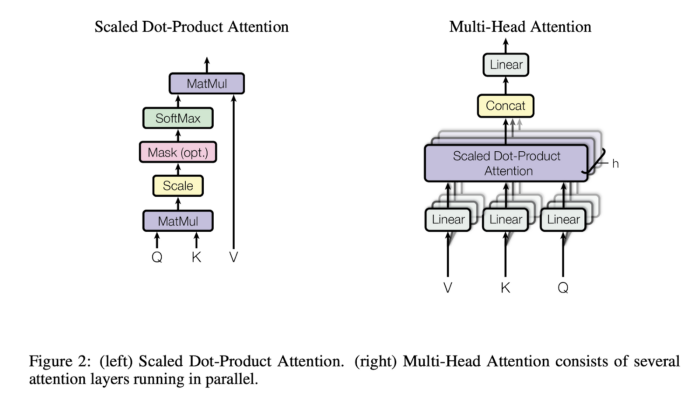
\includegraphics[width=\textwidth,height=\textheight,keepaspectratio]{02-03.png}
    \caption{The Attention Mechanism}
    \label{fig:attention}
\end{figure}

There are several advantages of attention layers over recurrent and convolutional networks, the two most important being their lower computational complexity and their higher connectivity, especially useful for learning long-term dependencies in sequences.

\subsection{What are Transformers used for and why are they so popular}

The original transformer was designed for language translation, particularly from English to German. But, already the original paper showed that the architecture generalized well to other language tasks. This particular trend became quickly noticed by the research community. Over the next few months most of the leaderboards for any language-related ML task became completely dominated by some version of the transformer architecture (see for example the well known SQUAD leaderboard\footnote{\url{https://rajpurkar.github.io/SQuAD-explorer/}} for question answer where all models at the top are ensembles of Transformers).

One of the key reasons Transformers were able to so quickly take over most NLP leaderboards is their ability to quickly adapt to other tasks, a.k.a. Transfer learning. Pretrained Transformer models can adapt extremely easily and quickly to tasks they have not been trained on, and that has huge advantages. As an ML practitioner, you no longer need to train a large model on a huge dataset. All you need to do is re-use the pretrained model on your task, maybe just slightly adapting it with a much smaller data set. A specific technique used to adapt pretrained models to a different task is the so-called fine tuning\footnote{\url{https://huggingface.co/docs/transformers/training}}.

It turns out that the capability of Transformers to adapt to other tasks is so great, that, while they were initially developed for language related tasks, they quickly became useful for other tasks ranging from vision\cite{khan2022transformers} or audio and music\footnote{\url{https://magenta.tensorflow.org/music-transformer}} applications all the way to playing chess\cite{noever2020chess} or doing math\cite{noorbakhsh2021pretrained}.

Of course all these applications would have not been possible if it wasn’t because of the myriad of tools that made them readily available to anyone that could write a few lines of code. Not only were Transformers quickly integrated into the main AI frameworks (namely Pytorch\footnote{\url{https://pytorch.org/tutorials/beginner/transformer_tutorial.html}} and TF\footnote{\url{https://www.tensorflow.org/text/tutorials/transformer}}), but they even enabled the creation of an entire company around them. Huggingface\footnote{\url{https://huggingface.co/docs}}, a startup that has raised over \$ 60M to this day, is almost entirely built around the idea of commercializing their open source Transformers library\footnote{\url{https://github.com/huggingface/transformers}}.

Last but not least, I would be remiss if I did not mention the impact of GPT-3\cite{brown2020language} on the popularization of Transformers. GPT-3 is a Transformer model introduced by OpenAI in May 2020 as a follow up to their earlier GPT and GPT-2. The company made a big splash by introducing the model in a preprint\cite{brown2020language} in which they claimed that the model was so powerful that they were not in a position to release it to the world. Since then, the model has not only been released, but also commercialized through a very large partnership\footnote{\url{https://openai.com/blog/openai-licenses-gpt-3-technology-to-microsoft/}} between OpenAI and Microsoft. GPT-3 powers over 300 different applications\footnote{\url{https://openai.com/blog/gpt-3-apps/}}, and is the foundation for OpenAI’s commercial strategy (which is a lot to say for a company that has received over \$ 1B in funding).

\subsection{RLHF}

Reinforcement Learning from Human Feedback (or Preferences) aka RLHF (or RLHP) has become a huge addition to the AI toolkit as of lately. The concept was introduced already in 2017 in the paper [“Deep reinforcement learning from human preferences”](https://arxiv.org/abs/1706.03741). More recently though, it has been applied to ChatGPT and similar dialog agents like BlenderBot3 or Sparrow. The idea is pretty simple though: Once a language model is pretrained, we can generate different responses to a dialog and have Humans rank the results. We can use those ranking (aka preferences or feedback) to train a reward, in the reinforcement learning context (see Figure \ref{fig:rlhf}). You can read much more in these two wonderful posts by Huggingface]\footnote{\url{https://huggingface.co/blog/rlhf}} or Weights and Bias\footnote{\url{https://wandb.ai/ayush-thakur/RLHF/reports/Understanding-Reinforcement-Learning-from-Human-Feedback-RLHF-Part-1--VmlldzoyODk5MTIx}}.

\begin{figure}
    \centering
    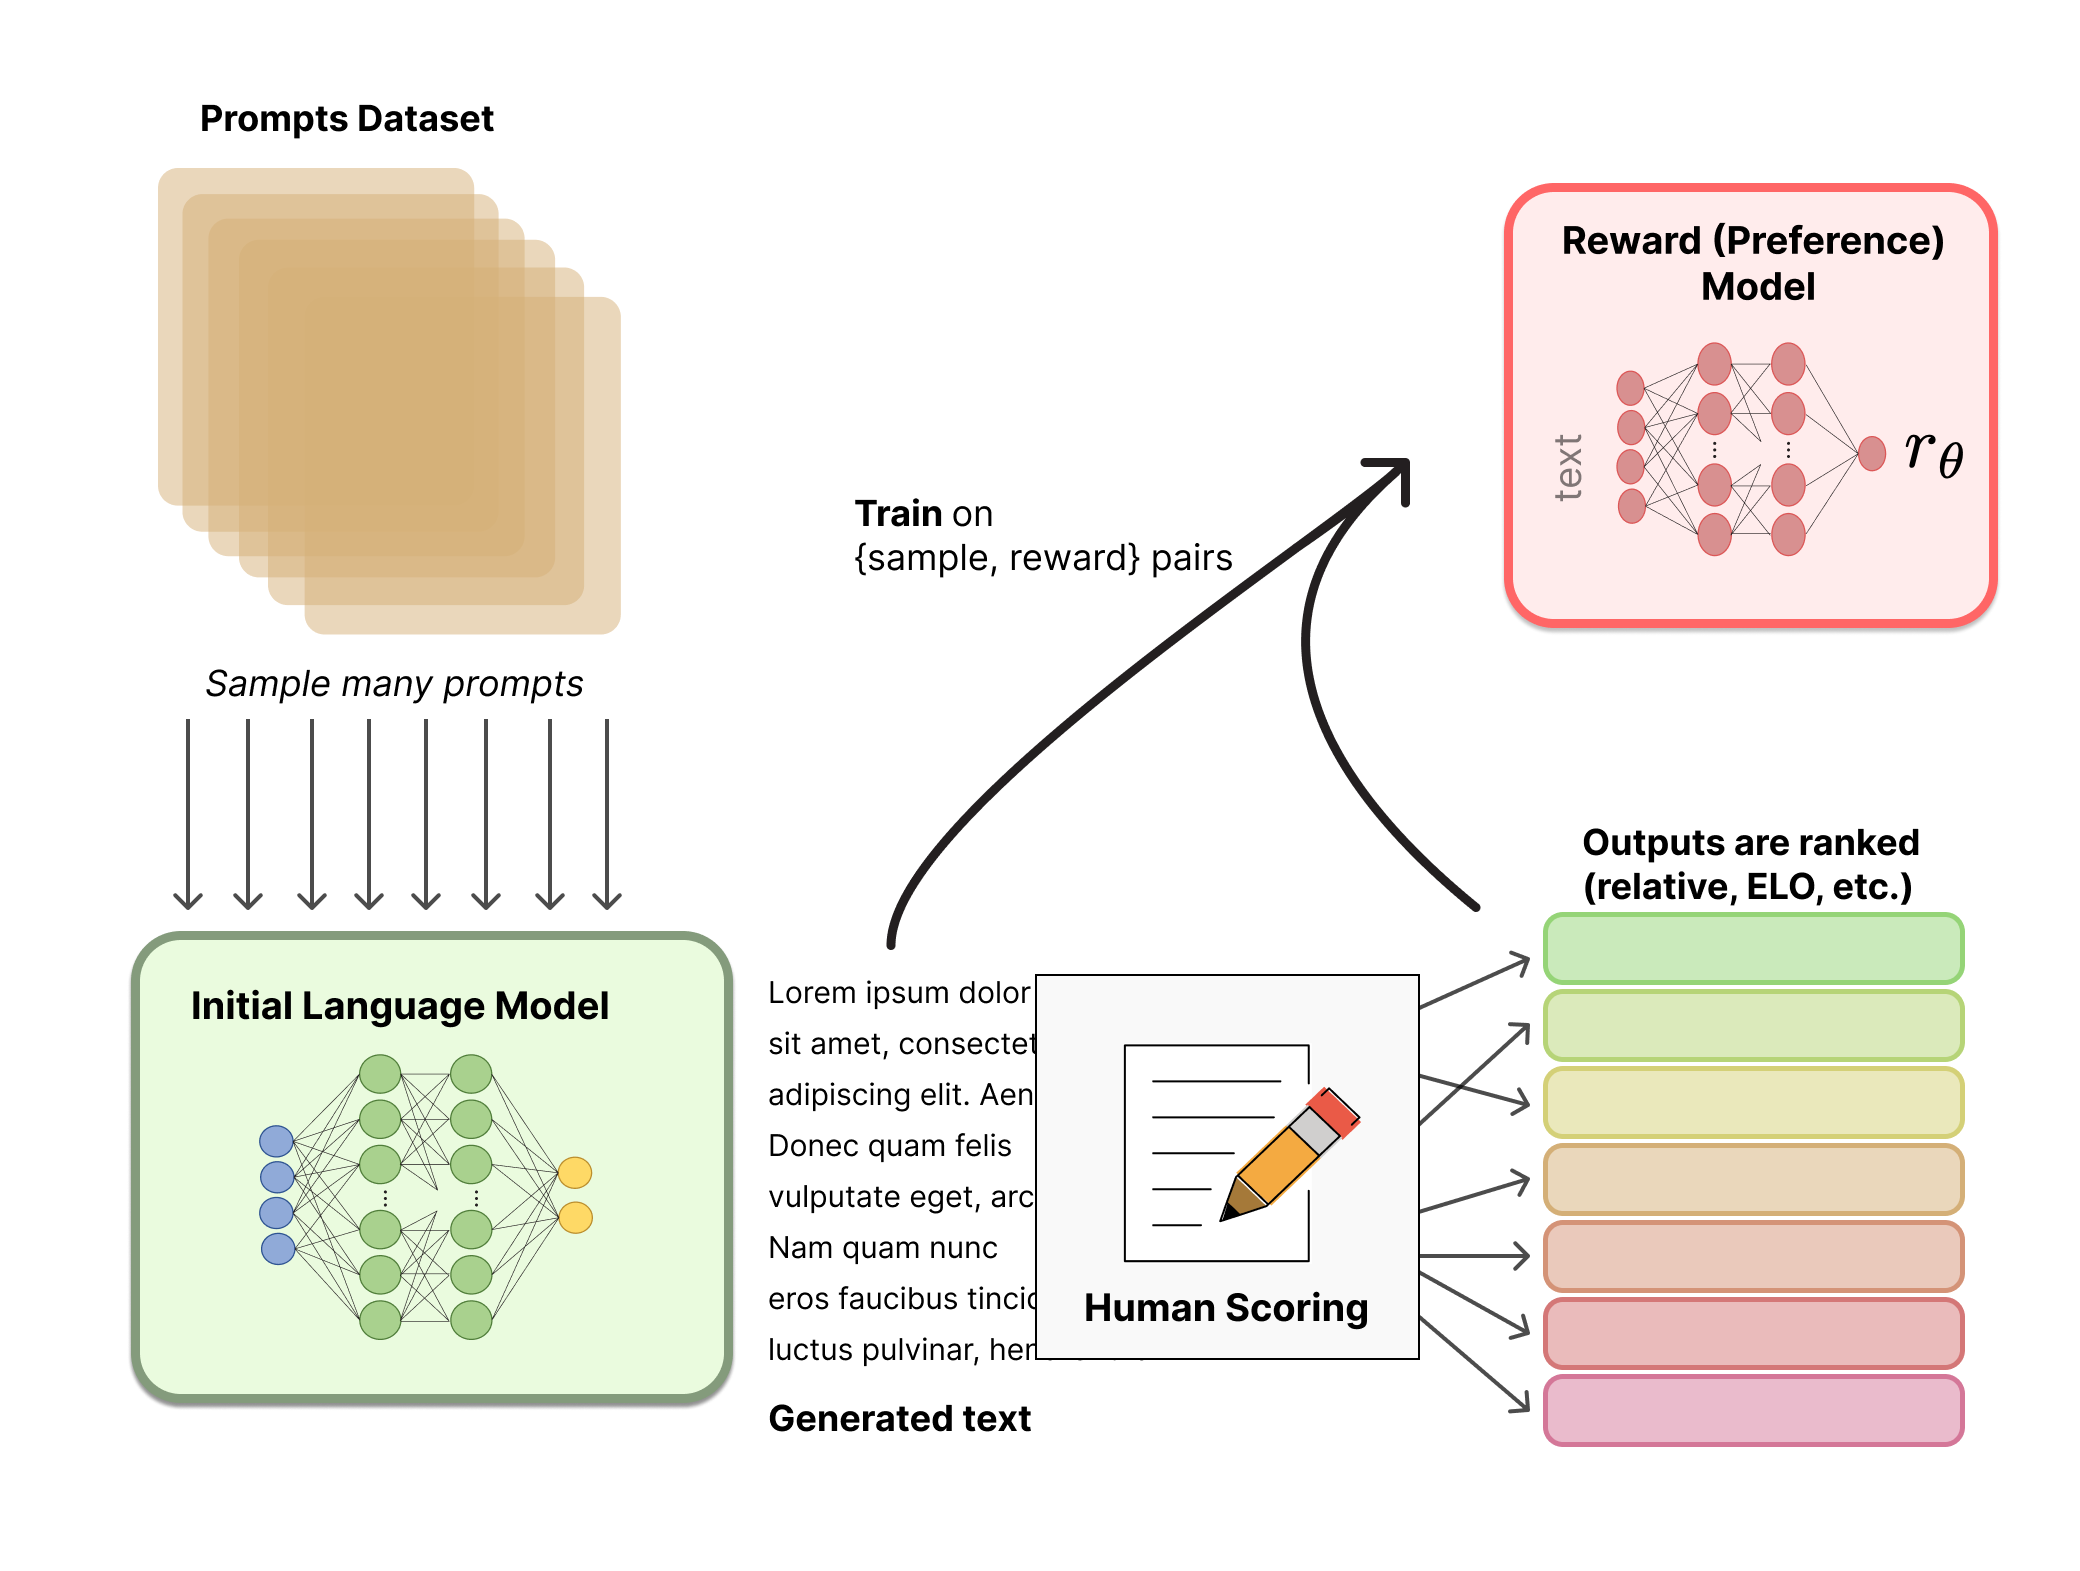
\includegraphics[width=\textwidth,height=\textheight,keepaspectratio]{rlhf.png}
    \caption{Reinforcement Learning with Human Feedback. From HuggingFace’s RLHF blog post at \url{https://huggingface.co/blog/rlhf}. }
    \label{fig:rlhf}
\end{figure}



\subsection{Diffusion}

Diffusion models have become the new SOTA in image generation, clearly pushing aside the previous approaches such as GANs (Generative Adversarial Networks). What are diffusion models? They are a class of latent variable models trained variational inference. What this means in practice is that we train a deep neural network to denoise images blurred with some sort of noise function. Networks that are trained this way are in fact learning the latent space of what those images represent (see figure \ref{fig:diffusion}.

\begin{figure}
    \centering
    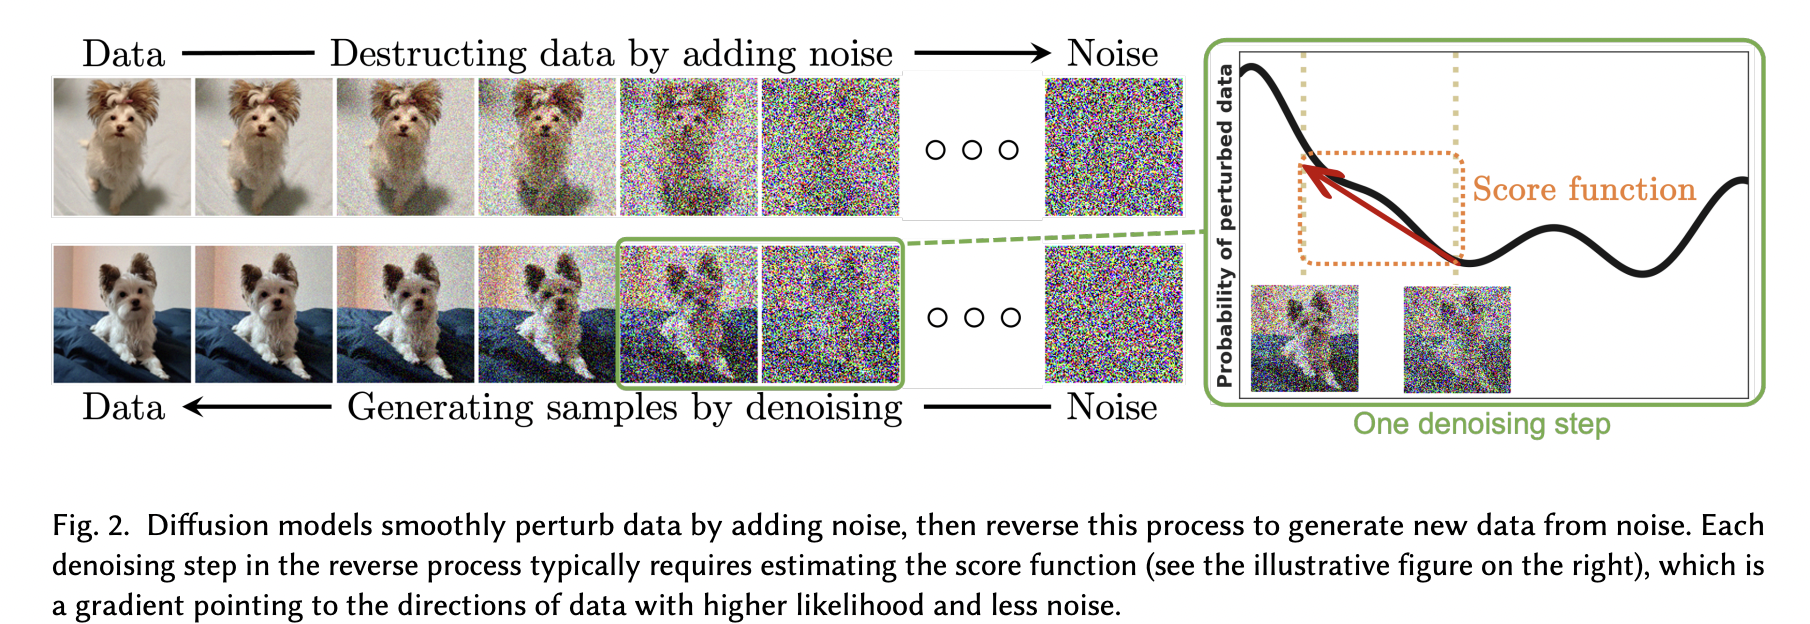
\includegraphics[width=\textwidth,height=\textheight,keepaspectratio]{diffusion.png}
    \caption{Probabilistic diffusion model architecture from “Diffusion Models: A Comprehensive Survey of Methods and Applications” \cite{yang2022diffusion} }
    \label{fig:diffusion}
\end{figure}


Diffusion models have relation with other generative models like the famous [Generative Adversarial Networks (GAN)]\footnote{\url{https://en.wikipedia.org/wiki/Generative_adversarial_network}}, which they have mostly replaced in many applications and, particularly with (denoising) Autoencoders. Some authors\footnote{\url{https://benanne.github.io/2022/01/31/diffusion.html}} will go as far as saying that Diffusion models are just a specific instance of autoencoders. However, they also admit that the small differences do transform their application, from the latent representation of autoconders to the pure generative nature of Diffusion models.

\section{The Transformers catalog}

\textbf{Note:} For all the models available in Huggingface, I decided to directly link to the page in the documentation since they do a fantastic job of offering a consistent format and links to everything else you might need, including the original papers. Only a few of the models are not included in Huggingface. For those, I try to include a link to their github if available or blog post if not. For all, I also include bibliographic reference.


\subsection{Features of a Transformer}

So hopefully by now you understand what Transformer models are, and why they are so popular and impactful. In this section I will introduce a catalog of the most important Transformer models that have been developed to this day. I will categorize each model according to the following properties: Pretraining Architecture, Pretraining Task, Compression, Application, Year, and Number of Parameters. Let’s briefly define each of those:

\subsubsection{Pretraining Architecture}

We described the Transformer architecture as being made up of an Encoder and a Decoder, and that is true for the original Transformer. However, since then, different advances have been made that have revealed that in some cases it is beneficial to use only the encoder, only the decoder, or both.

\paragraph{Encoder Pretraining}

These models, which are also called bi-directional or auto-encoding, only use the encoder during pretraining, which is usually accomplished by masking words in the input sentence and training the model to reconstruct. At each stage during pretraining, attention layers can access all the input words. This family of models are most useful for tasks that require understanding complete sentences such as sentence classification or extractive question answering.

\paragraph{Decoder Pretraining}

Decoder models, often called auto-regressive, use only the decoder during a pretraining that is usually designed so the model is forced to predict the next word. The attention layers can only access the words positioned before a given word in the sentence. They are best suited for tasks involving text generation.

\paragraph{Transformer (Encoder-Decoder) Pretraining}

Encoder-decoder models, also called sequence-to-sequence, use both parts of the Transformer architecture. Attention layers of the encoder can access all the words in the input, while those of the decoder can only access the words positioned before a given word in the input. The pretraining can be done using the objectives of encoder or decoder models, but usually involves something a bit more complex. These models are best suited for tasks revolving around generating new sentences depending on a given input, such as summarization, translation, or generative question answering.

\subsubsection{Pretraining Task}

When training a model we need to define a task for the model to learn on. Some of the typical tasks, such as predicting the next word or learning to reconstruct masked words were already mentioned above. “Pre-trained Models for Natural Language Processing: A Survey”\cite{qiu2020pre} includes a pretty comprehensive taxonomy of pretraining tasks, all of which can be considered self-supervised:

\begin{enumerate}
    \item \textbf{Language Modeling (LM):} Predict next token (in the case of unidirectional LM) or previous and next token (in the case of bidirectional LM)
    \item \textbf{Masked Language Modeling (MLM):} mask out some tokens from the input sentences and then trains the model to predict the masked tokens by the rest of the tokens
    \item \textbf{Permuted Language Modeling (PLM):} same as LM but on a random permutation of input sequences. A permutation is randomly sampled from all possible permutations. Then some of the tokens are chosen as the target, and the model is trained to predict these targets.
    \item \textbf{Denoising Autoencoder (DAE):} take a partially corrupted input (e.g. Randomly sampling tokens from the input and replacing them with "[MASK]" elements. randomly deleting tokens from the input, or shuffling sentences in random order) and aim to recover the original undistorted input.
    \item \textbf{Contrastive Learning (CTL):} A score function for text pairs is learned by assuming some observed pairs of text that are more semantically similar than randomly sampled text. It includes: 
    \begin{itemize}
       \item \textbf{Deep InfoMax (DIM):} maximize mutual information between an image representation and local regions of the image; 
       \item \textbf{Replaced Token Detection (RTD):} predict whether a token is replaced given its surroundings; 
       \item \textbf{Next Sentence Prediction (NSP):} train the model to distinguish whether two input sentences are continuous segments from the training corpus; and 
       \item \textbf{Sentence Order Prediction (SOP):} Similar to NSP, but uses two consecutive segments as positive examples, and the same segments but with their order swapped as negative examples
   \end{itemize} 
   
\end{enumerate}

\subsubsection{Application}

Here we will note what are the main practical applications of the Transformer model. Most of these applications will be in the language domain (e.g. question answering, sentiment analysis, or entity recognition). However, as mentioned before, some Transformer models have also found applications well beyond NLP and are also included in the catalog.

\subsection{Catalog table}

Figure \ref{fig:table} is a screenshot of a large table where I have tabulated all the models. If you are interested in the table, access it directly in \footnote{\url{https://docs.google.com/spreadsheets/d/1ltyrAB6BL29cOv2fSpNQnnq2vbX8UrHl47d7FkIf6t4}}

\begin{figure}
    \centering
    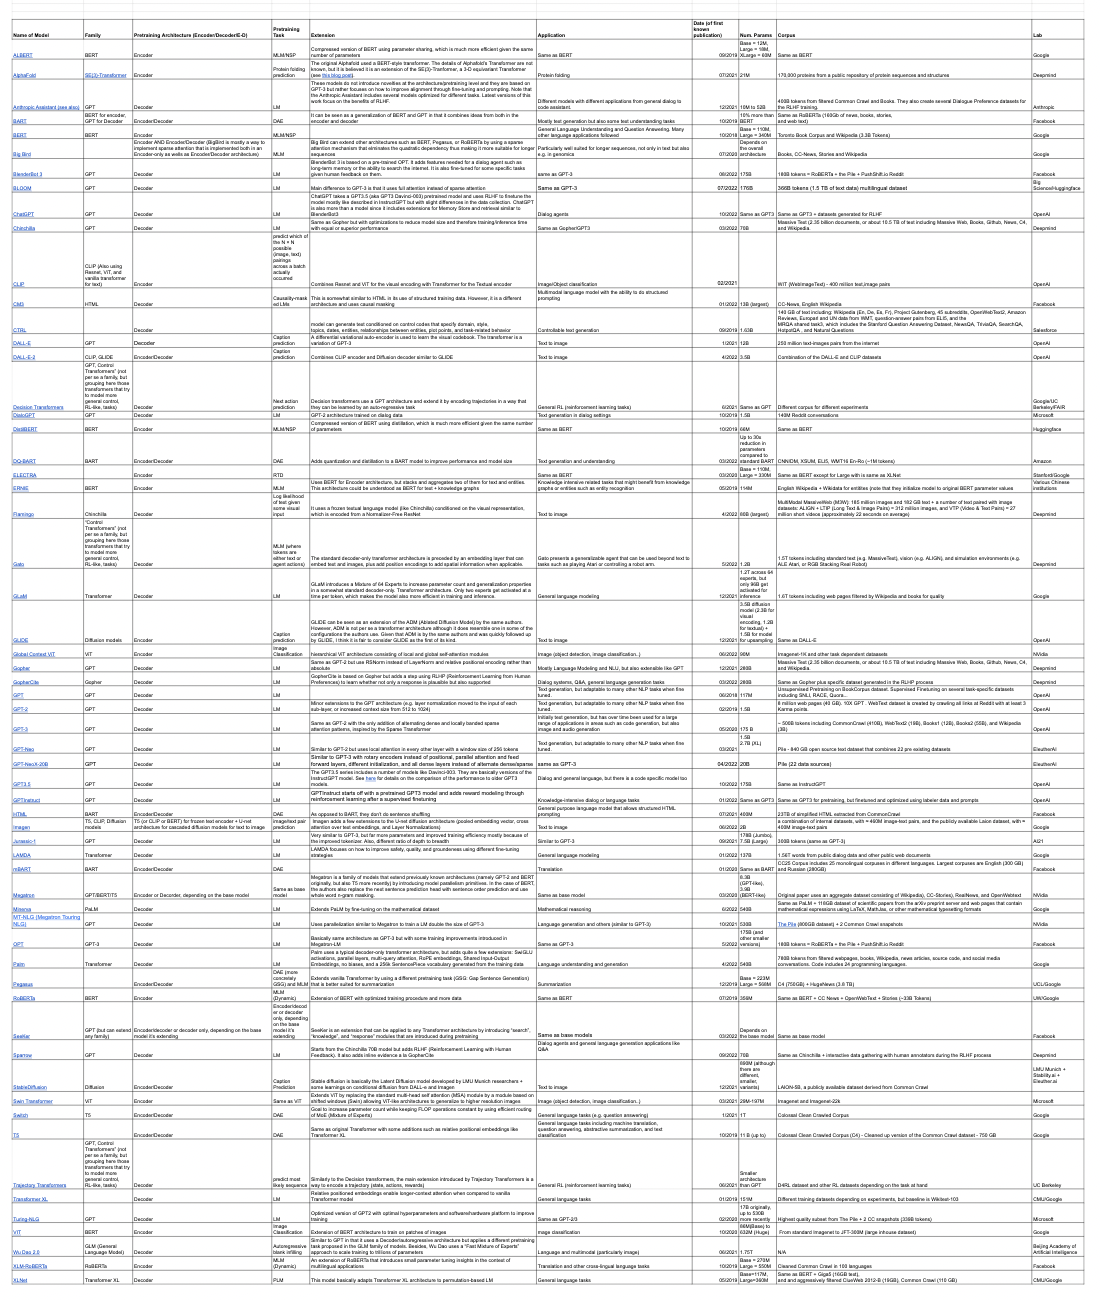
\includegraphics[width=\textwidth,height=\textheight,keepaspectratio]{02-04.png}
    \caption{You can access the original table at \url{https://docs.google.com/spreadsheets/d/1ltyrAB6BL29cOv2fSpNQnnq2vbX8UrHl47d7FkIf6t4} for easier browsing across the different model features.}
    \label{fig:table}
\end{figure}

\subsection{Family Tree}

The diagram in figure \ref{fig:tree} is a simple view that highlights the different families of transformers and how they relate to each other.

\begin{figure}
    \centering
    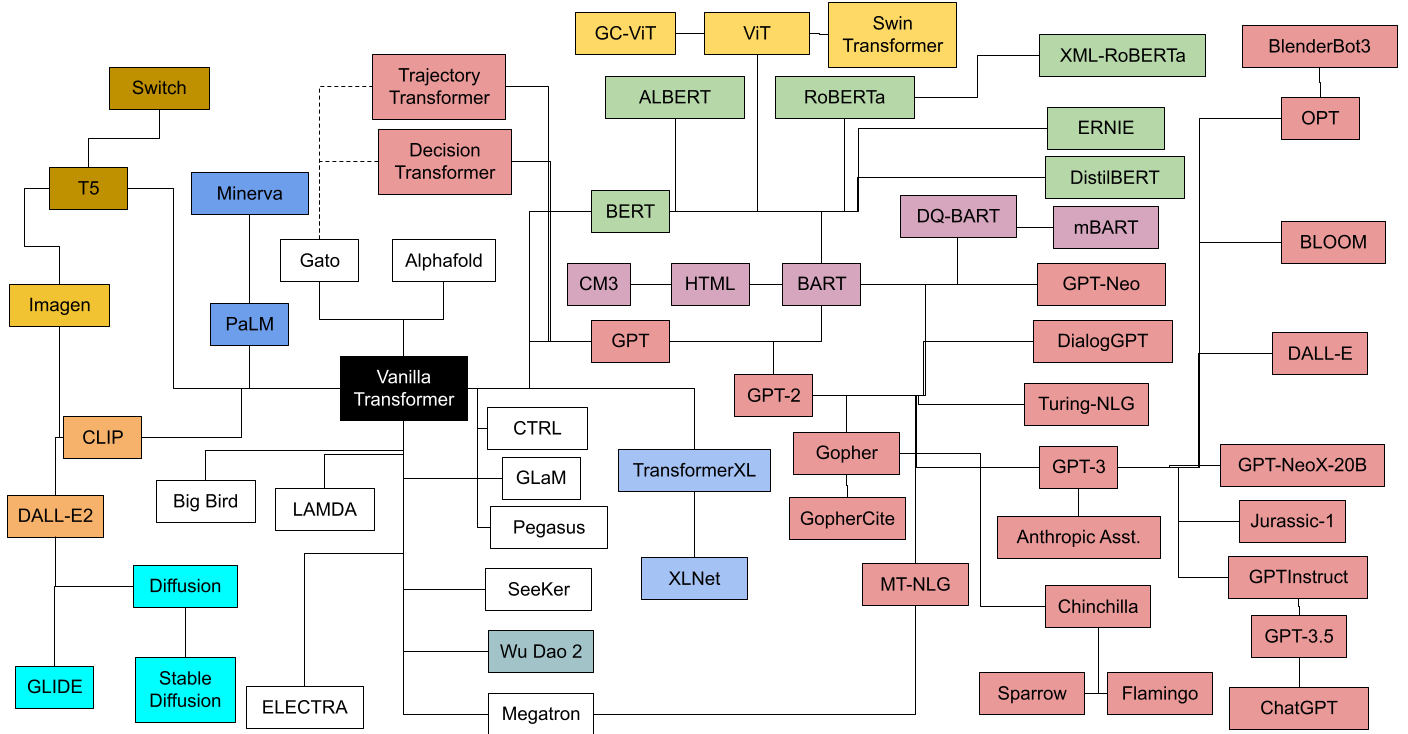
\includegraphics[width=\textwidth,height=\textheight,keepaspectratio]{02-05.png}
    \caption{}
    \label{fig:tree}
\end{figure}

\subsection{Chronological timeline}

Another interesting perspective of the catalog is to see it as a chronological timeline. In Figure \ref{fig:timeline} you will find all the transformers in the catalog sorted by their date of publication. In this first visualization, the Y-axis is only used to cluster transformers of related heritage/family.

\begin{figure}
    \centering
    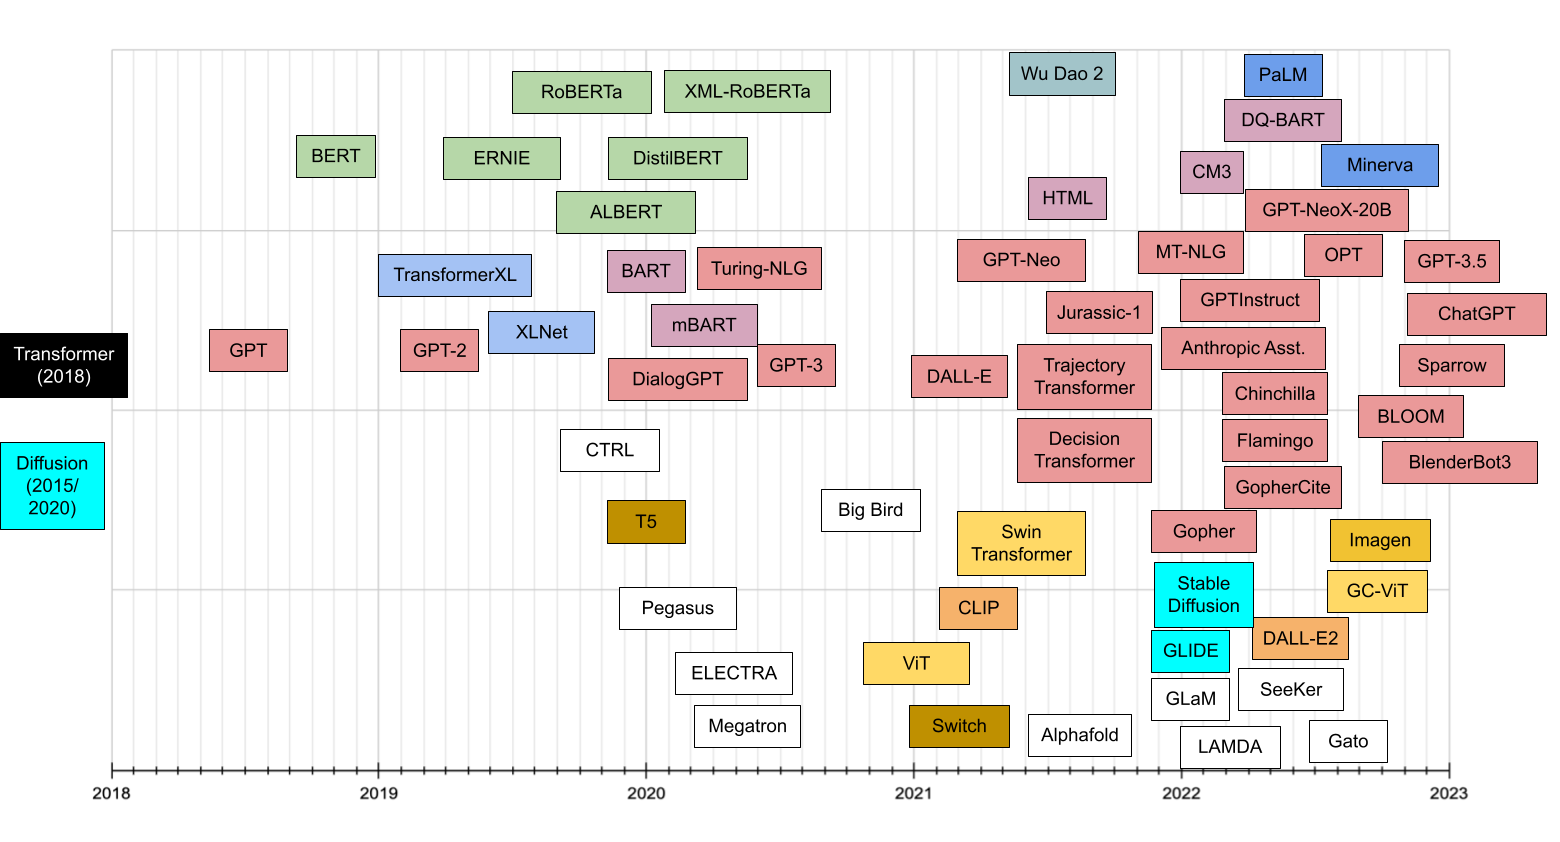
\includegraphics[width=\textwidth,height=\textheight,keepaspectratio]{02-06.png}
    \caption{Transformer timeline. Colors describe Transformer family.}
    \label{fig:timeline}
\end{figure}

In Figure \ref{fig:timelineSize}, the Y-axis represents model size in millions of parameters. You won't be able to see all the models in the catalog since many fall right on the same time and size, so please refer to the previous image for that.

\begin{figure}
    \centering
    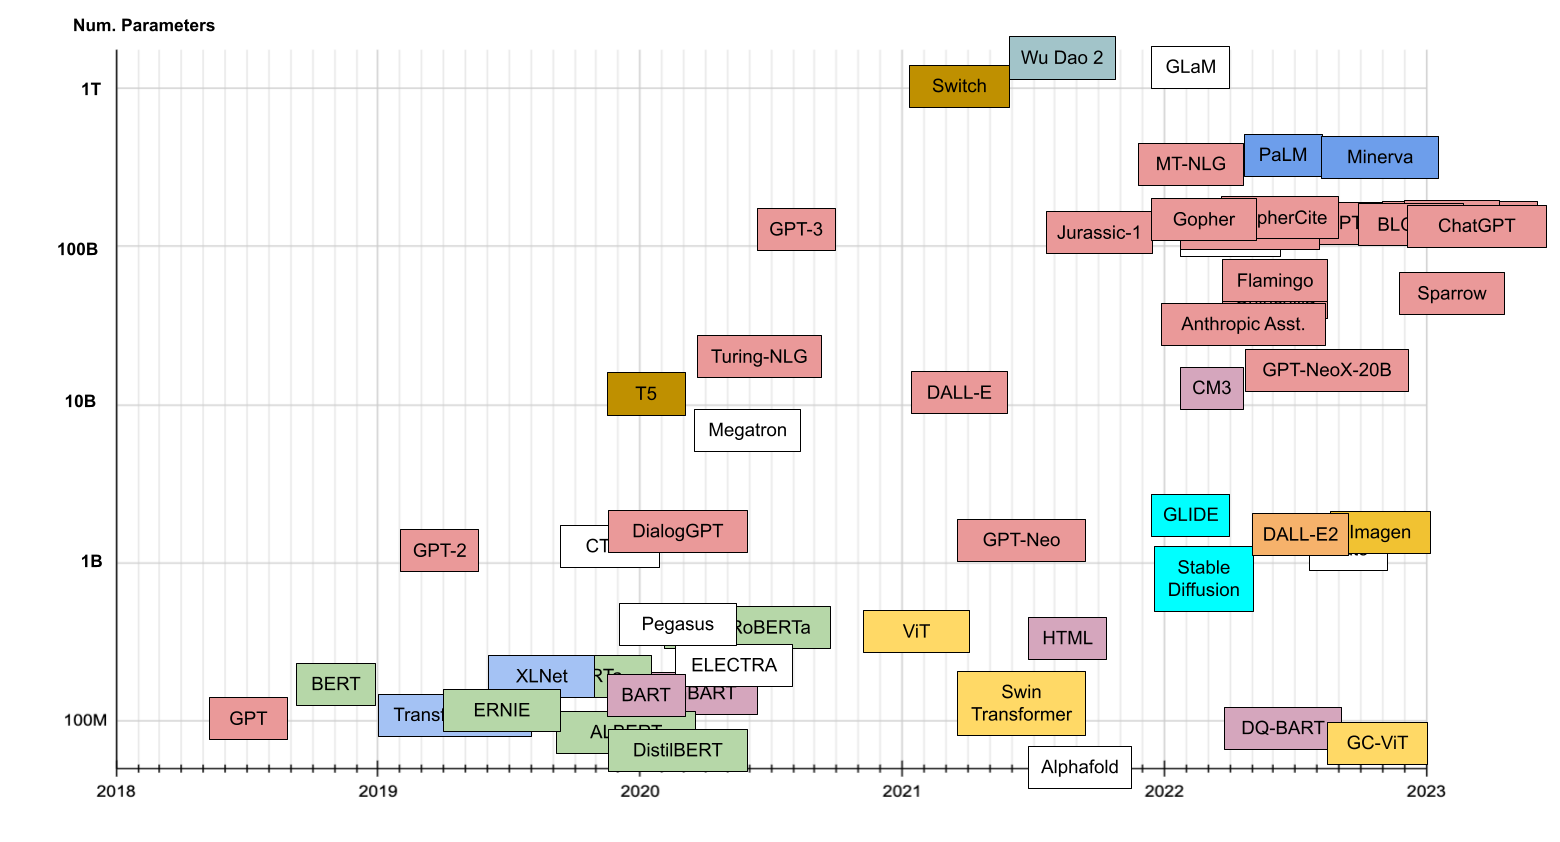
\includegraphics[width=\textwidth,height=\textheight,keepaspectratio]{02-09.png}
    \caption{Transformer timeline. On the vertical axis, number of parameters. Colors describe Transformer family.}
    \label{fig:timelineSize}
\end{figure}

\subsection{Catalog List}

Finally, here is the full list view that might be easier to follow along in some cases:

\subsubsection{ALBERT}
            \begin{itemize}
                \item \textbf{Reference:}\footnote{\url{https://huggingface.co/docs/transformers/model_doc/albert}}\cite{lan2019albert}
                \item \textbf{Family:} BERT
                \item \textbf{Pretraining Architecture:} Encoder
                \item \textbf{Pretraining Task:} MLM/NSP
                \item \textbf{Extension:} Compressed version of BERT using parameter sharing, which is much more efficient given the same number of parameters
                \item \textbf{Application:} Same as BERT
                \item \textbf{Date (of first known publication):} 09/2019
                \item \textbf{Num. Params:}b12M, Large = 18M, XLarge = 60M*
                \item \textbf{Corpus:}Same as BERT
                \item \textbf{Lab:} Google
            \end{itemize}

\subsubsection{AlphaFold}
            \begin{itemize}
                \item \textbf{Reference:}\footnote{\url{https://www.deepmind.com/publications/highly-accurate-protein-structure-prediction-with-alphafold}}\cite{jumper2021highly}
                \item \textbf{Family:} SE(3) Transformer\footnote{\url{https://arxiv.org/abs/2006.10503}}
                \item \textbf{Pretraining Architecture:} Encoder
                \item \textbf{Pretraining Task:} Protein folding prediction*ion of BERT using parameter sharing, which is much more efficient given the same number of parameters
                \item \textbf{Extension:}The original Alphafold used a BERT-style transformer. The details of Alphafold’s Transformer are not known, but it is believed it is an extension of the SE(3)-Tranformer, a 3-D equivariant Transformer (see this blog post\footnote{\url{https://fabianfuchsml.github.io/alphafold2/}})   
                \item \textbf{Application:} Same as BERT
                \item \textbf{Date (of first known publication):} 09/2019
                \item \textbf{Num. Params:}b12M, Large = 18M, XLarge = 60M*
                \item \textbf{Corpus:}Same as BERT
                \item \textbf{Lab:}Google
            \end{itemize}
            
\subsubsection{Anthropic Assistant}

            \begin{itemize}
                \item \textbf{Reference:}\footnote{\url{https://arxiv.org/abs/2112.00861}} see also\footnote{\url{https://arxiv.org/abs/2204.05862}} \cite{bai2022training,askell2021general}
                \item \textbf{Family:} GPT 
                \item \textbf{Pretraining Architecture:} Decoder
                \item \textbf{Pretraining Task:} Protein folding prediction*ion of BERT using parameter sharing, which is much more efficient given the same number of parameters
                \item \textbf{Extension:These models do not introduce novelties at the architecture/pretraining level and they are based on GPT-3 but rather focuses on how to improve alignment through fine-tuning and prompting. Note that the Anthropic Assistant includes several models optimized for different tasks. Latest versions of this work focus on the benefits of RLHF}   
                \item \textbf{Application:} Different models with different applications from general dialog to code assistant.
                \item \textbf{Date (of first known publication):} 12/2021
                \item \textbf{Num. Params:}10M to 52B
                \item \textbf{Corpus:}400B tokens from filtered Common Crawl and Books. They also create several Dialogue Preference datasets for the RLHF training.
                \item \textbf{Lab:}Anthropic
            \end{itemize}

\subsubsection{BART}
            \begin{itemize}
                \item \textbf{Reference:}\footnote{\url{https://huggingface.co/docs/transformers/model_doc/bart}}\cite{lewis2019bart}
                \item \textbf{Family:} BERT for encoder, GPT for Decoder 
                \item \textbf{Pretraining Architecture:} Encoder/Decoder
                \item \textbf{Pretraining Task:} DAE
                \item \textbf{Extension:It can be seen as a generalization of BERT and GPT in that it combines ideas from both in the encoder and decoder}   
                \item \textbf{Application:} Mostly text generation but also some text understanding tasks*
                \item \textbf{Date (of first known publication):} 10/2019*
                \item \textbf{Num. Params:}10 \% more than BERT
                \item \textbf{Corpus:}Same as RoBERTa (160Gb of news, books, stories
                \item \textbf{Lab:}Facebook
            \end{itemize}

\subsubsection{BERT}

            \begin{itemize}
                \item \textbf{Reference:}\footnote{\url{https://huggingface.co/docs/transformers/model_doc/bert}}\cite{devlin2018bert}
                \item \textbf{Family:} BERT 
                \item \textbf{Pretraining Architecture:} Encoder
                \item \textbf{Pretraining Task:} MLM/NSP
                \item \textbf{Extension:It can be seen as a generalization of BERT and GPT in that it combines ideas from both in the encoder and decoder}   
                \item \textbf{Application:}General Language Understanding and Question Answering. Many other language applications followed
                \item \textbf{Date (of first known publication):} 10/2018
                \item \textbf{Num. Params:}Base = 110M, Large = 340MT
                \item \textbf{Corpus:}Toronto Book Corpus and Wikipedia (3.3B Tokens)
                \item \textbf{Lab:}Google
            \end{itemize}

\subsubsection{Big Bird}

            \begin{itemize}
                \item \textbf{Reference:}\footnote{\url{https://huggingface.co/docs/transformers/model_doc/big_bird}}\cite{zaheer2020big}
                \item \textbf{Family:} BERT 
                \item \textbf{Pretraining Architecture:} Encoder
                \item \textbf{Pretraining Task:} MLM
                \item \textbf{Extension:} Big Bird can extend other architectures such as BERT, Pegasus, or RoBERTa by using a sparse attention mechanism that elminates the quadratic dependency thus making it more suitable for longer sequences 
                \item \textbf{Application:}Particularly well suited for longer sequences, not only in text but also e.g. in genomics
                \item \textbf{Date (of first known publication):} 07/2020
                \item \textbf{Num. Params:}Depends on the overall architecture
                \item \textbf{Corpus:}Books, CC-News, Stories and Wikipedia)
                \item \textbf{Lab:}Google
            \end{itemize}

\subsubsection{BlenderBot3}

            \begin{itemize}
                \item \textbf{Reference:}\footnote{\url{https://arxiv.org/abs/2208.03188}}\cite{shuster2022blenderbot}
                \item \textbf{Family:} GPT 
                \item \textbf{Pretraining Architecture:} Decoder
                \item \textbf{Pretraining Task:} LM
                \item \textbf{Extension:} BlenderBot 3 is based on a pre-trained OPT. It adds features needed for a dialog agent such as long-term memory or the ability to search the internet. It is also fine-tuned for some specific tasks given human feedback on them.  
                \item \textbf{Application:} Same as GPT-3
                \item \textbf{Date (of first known publication):} 08/2022
                \item \textbf{Num. Params:}175B
                \item \textbf{Corpus:} 180B tokens = RoBERTa + the Pile + PushShift.io Reddit
                \item \textbf{Lab:}Facebook
            \end{itemize}

\subsubsection{BLOOM}
            \begin{itemize}
                \item \textbf{Reference:}\footnote{\url{https://huggingface.co/docs/transformers/model_doc/bloom}}
                \item \textbf{Family:} GPT 
                \item \textbf{Pretraining Architecture:} Decoder
                \item \textbf{Pretraining Task:} LM
                \item \textbf{Extension:} Main difference to GPT-3 is that it uses full attention instead of sparse attention  
                \item \textbf{Application:} Same as GPT-3
                \item \textbf{Date (of first known publication):} 07/2022
                \item \textbf{Num. Params:}176B
                \item \textbf{Corpus:} 366B tokens (1.5 TB of text data) multilingual dataset
                \item \textbf{Lab:} Big Science/Huggingface
            \end{itemize}
            
\subsubsection{ChatGPT}

            \begin{itemize}
                \item \textbf{Reference:}\footnote{\url{https://openai.com/blog/chatgpt/}}
                \item \textbf{Family:} GPT 
                \item \textbf{Pretraining Architecture:} Decoder
                \item \textbf{Pretraining Task:} LM
                \item \textbf{Extension:} ChatGPT takes a GPT3.5 (aka GPT3 Davinci-003) pretrained model and uses RLHF to finetune the model mostly like described in InstructGPT but with slight differences in the data collection. ChatGPT is also more than a model since it includes extensions for Memory Store and retrieval similar to BlenderBot3  
                \item \textbf{Application:} Dialog agents
                \item \textbf{Date (of first known publication):} 10/2022
                \item \textbf{Num. Params:}Same as GPT3
                \item \textbf{Corpus:} Same as GPT3 + datasets generated for RLHF
                \item \textbf{Lab:} OpenAI
            \end{itemize}

\subsubsection{Chinchilla}

            \begin{itemize}
                \item \textbf{Reference:}\footnote{\url{https://arxiv.org/abs/2203.15556}}\cite{hoffmann2022training}
                \item \textbf{Family:} GPT 
                \item \textbf{Pretraining Architecture:} Decoder
                \item \textbf{Pretraining Task:} LM
                \item \textbf{Extension:} Same as Gopher but with optimizations to reduce model size and therefore training/inference time with equal or superior performance  
                \item \textbf{Application:} Same as Gopher/GPT3
                \item \textbf{Date (of first known publication):} 03/2022
                \item \textbf{Num. Params:}70B
                \item \textbf{Corpus:} Massive Text
                \item \textbf{Lab:} Deepmind
            \end{itemize}

\subsubsection{CLIP}

            \begin{itemize}
                \item \textbf{Reference:}\footnote{\url{https://huggingface.co/docs/transformers/model_doc/clip}}\cite{radford2021learning}
                \item \textbf{Family:} CLIP (Also using Resnet, ViT, and vanilla transformer for text) 
                \item \textbf{Pretraining Architecture:} Encoder
                \item \textbf{Pretraining Task:} predict which of the N × N possible (image, text) pairings across a batch actually occurred
                \item \textbf{Extension:} Combines Resnet and ViT for the visual encoding with Transformer for the Textual encoder  
                \item \textbf{Application:} Image/object classification
                \item \textbf{Date (of first known publication):} 02/2021
                \item \textbf{Num. Params:}?
                \item \textbf{Corpus:} WIT (WebImageText) - 400 million text,image pairs
                \item \textbf{Lab:} OpenAI
            \end{itemize}     
            
\subsubsection{CM3}

            \begin{itemize}
                \item \textbf{Reference:}\footnote{\url{https://arxiv.org/abs/2201.07520}}\cite{aghajanyan2022cm3}
                \item \textbf{Family:} HTML 
                \item \textbf{Pretraining Architecture:} Decoder
                \item \textbf{Pretraining Task:} Causality-masked LM
                \item \textbf{Extension:} This is somewhat similar to HTML in its use of structured training data. However, it is a different architecture and uses causal masking  
                \item \textbf{Application:} Multimodal language model with the ability to do structured prompting
                \item \textbf{Date (of first known publication):} 01/2022
                \item \textbf{Num. Params:}13B (largest)
                \item \textbf{Corpus:} CC-News, English Wikipedia
                \item \textbf{Lab:} Facebook
            \end{itemize}

\subsubsection{CTRL}

            \begin{itemize}
                \item \textbf{Reference:}\footnote{\url{https://huggingface.co/docs/transformers/model_doc/ctrl}}\cite{keskar2019ctrl}
                \item \textbf{Family:} 
                \item \textbf{Pretraining Architecture:} Decoder
                \item \textbf{Pretraining Task:}
                \item \textbf{Extension:} model can generate text conditioned on control codes that specify domain, style, topics, dates, entities, relationships between entities, plot points, and task-related behavior  
                \item \textbf{Application:} Controllable text generation
                \item \textbf{Date (of first known publication):} xx
                \item \textbf{Num. Params:}1.63B
                \item \textbf{Corpus:} 140 GB of text including: Wikipedia (En, De, Es, Fr), Project Gutenberg, 45 subreddits, OpenWebText2, Amazon Reviews, Europarl and UN data from WMT, question-answer pairs from ELI5, and the MRQA shared task3, which includes the Stanford Question Answering Dataset, NewsQA, TriviaQA, SearchQA, HotpotQA , and Natural Questions
                \item \textbf{Lab:} Salesforce
            \end{itemize}
            
\subsubsection{DALL-E}

            \begin{itemize}
                \item \textbf{Reference:}\footnote{\url{https://openai.com/blog/dall-e/}}\cite{ramesh2021zero}
                \item \textbf{Family:} GPT 
                \item \textbf{Pretraining Architecture:} Decoder
                \item \textbf{Pretraining Task:} Caption prediction
                \item \textbf{Extension:} A differential variational auto-encoder is used to learn the visual codebook. The transformer is a variation of GPT-3  
                \item \textbf{Application:} Text to image
                \item \textbf{Date (of first known publication):} 01/2021
                \item \textbf{Num. Params:}12B
                \item \textbf{Corpus:} 250 million text-images pairs from the internet
                \item \textbf{Lab:} OpenAI
            \end{itemize}
            
\subsubsection{DALL-E 2}

            \begin{itemize}
                \item \textbf{Reference:}\footnote{\url{https://openai.com/dall-e-2/}}\cite{ramesh2022hierarchical}
                \item \textbf{Family:} CLIP, GLIDE 
                \item \textbf{Pretraining Architecture:} Encoder/Decoder
                \item \textbf{Pretraining Task:} Caption prediction
                \item \textbf{Extension:} Combines CLIP encoder and Diffusion decoder similar to GLIDE  
                \item \textbf{Application:} Text to image
                \item \textbf{Date (of first known publication):} 04/2022
                \item \textbf{Num. Params:}3.5B
                \item \textbf{Corpus:} Combination of the DALL-E and CLIP datasets
                \item \textbf{Lab:} OpenAI
            \end{itemize}

\subsubsection{Decision Transformers}

            \begin{itemize}
                \item \textbf{Reference:}\footnote{\url{https://arxiv.org/abs/2106.01345}}\cite{chen2021decision}
                \item \textbf{Family:} GPT, Control Transformers” (not per se a family, but grouping here those transformers that try to model more general control, RL-like, tasks) 
                \item \textbf{Pretraining Architecture:} Decoder
                \item \textbf{Pretraining Task:} Next action prediction
                \item \textbf{Extension:} Decision transformers use a GPT architecture and extend it by encoding trajectories in a way that they can be learned by an auto-regressive task  
                \item \textbf{Application:} General RL (reinforcement learning tasks)
                \item \textbf{Date (of first known publication):} 06/2021
                \item \textbf{Num. Params:}Same as GPT
                \item \textbf{Corpus:} Different corpus for different experiments
                \item \textbf{Lab:} Google/UC Berkeley/Facebook
            \end{itemize}

\subsubsection{DialoGPT}
            \begin{itemize}
                \item \textbf{Reference:}\footnote{\url{https://huggingface.co/docs/transformers/model_doc/dialogpt}}\cite{zhang2019dialogpt}
                \item \textbf{Family:} GPT 
                \item \textbf{Pretraining Architecture:} Decoder
                \item \textbf{Pretraining Task:} LM
                \item \textbf{Extension:} GPT-2 architecture trained on dialog data  
                \item \textbf{Application:} Text generation in dialog settings
                \item \textbf{Date (of first known publication):} 10/2019
                \item \textbf{Num. Params:}1.5B
                \item \textbf{Corpus:} 140M Reddit conversations
                \item \textbf{Lab:} Microsoft
            \end{itemize}
            
\subsubsection{DistilBERT}
            \begin{itemize}
                \item \textbf{Reference:}\footnote{\url{https://huggingface.co/docs/transformers/model_doc/distilbert}}\cite{sanh2019distilbert}
                \item \textbf{Family:} BERT 
                \item \textbf{Pretraining Architecture:} Encoder
                \item \textbf{Pretraining Task:} MLM/NSP
                \item \textbf{Extension:} Compressed version of BERT using distillation, which is much more efficient given the same number of parameters  
                \item \textbf{Application:} Same as BERT
                \item \textbf{Date (of first known publication):} 10/2019
                \item \textbf{Num. Params:}66M
                \item \textbf{Corpus:} Same as BERT
                \item \textbf{Lab:} Huggingface
            \end{itemize}
            
\subsubsection{DQ-BART}

            \begin{itemize}
                \item \textbf{Reference:}\footnote{\url{https://arxiv.org/abs/2203.11239}}\cite{li2022dq}
                \item \textbf{Family:} BART 
                \item \textbf{Pretraining Architecture:} Encoder/Decoder
                \item \textbf{Pretraining Task:} DAE
                \item \textbf{Extension:} Adds quantization and distillation to a BART model to improve performance and model size  
                \item \textbf{Application:} Text generation and understanding
                \item \textbf{Date (of first known publication):} 03/2022
                \item \textbf{Num. Params:}Up to 30x reduction in parameters compared to standard BART
                \item \textbf{Corpus:} CNN/DM, XSUM, ELI5, WMT16 En-Ro (~1M tokens)
                \item \textbf{Lab:} Amazon
            \end{itemize}

\subsubsection{ELECTRA}

            \begin{itemize}
                \item \textbf{Reference:}\footnote{\url{https://huggingface.co/docs/transformers/model_doc/electra}}\cite{clark2020electra}
                \item \textbf{Family:} 
                \item \textbf{Pretraining Architecture:} Encoder
                \item \textbf{Pretraining Task:} RTD
                \item \textbf{Extension:} Same as BERT  
                \item \textbf{Application:} 03/2020
                \item \textbf{Date (of first known publication):} xx
                \item \textbf{Num. Params:}Base = 110M, Large = 330M
                \item \textbf{Corpus:} Same as BERT except for Large with is same as XLNet
                \item \textbf{Lab:} Stanford/Google
            \end{itemize}

\subsubsection{ERNIE}

            \begin{itemize}
                \item \textbf{Reference:}\footnote{\url{https://arxiv.org/abs/1905.07129}}\cite{zhang2019ernie}
                \item \textbf{Family:} BERT 
                \item \textbf{Pretraining Architecture:} Encoder
                \item \textbf{Pretraining Task:} MLM
                \item \textbf{Extension:} Uses BERT for Encoder architecture, but stacks and aggregates two of them for text and entities. This architecture could be understood as BERT for text + knowledge graphs  
                \item \textbf{Application:} Knowledge intensive related tasks that might benefit from knowledge graphs or entities such as entity recognition
                \item \textbf{Date (of first known publication):} 05/2019
                \item \textbf{Num. Params:}114M
                \item \textbf{Corpus:} English Wikipedia + Wikidata for entitites (note that they initialize model to original BERT parameter values
                \item \textbf{Lab:} Various Chinese institutions
            \end{itemize} 

\subsubsection{FLAN T5}

            \begin{itemize}
                \item \textbf{Reference:}\footnote{\url{https://huggingface.co/docs/transformers/model_doc/flan-t5}}\cite{chung2022flan}
                \item \textbf{Family:} T5
                \item \textbf{Pretraining Architecture:} Encoder/Decoder
                \item \textbf{Pretraining Task:} DAE
                \item \textbf{Extension:} Same as T5 with additional general instruction finetuning
                \item \textbf{Application:} General language tasks including machine translation, question answering, abstractive summarization, and text classification
                \item \textbf{Date (of first known publication):} 10/2022
                \item \textbf{Num. Params:} 11 B (up to)
                \item \textbf{Corpus:} Colossal Clean Crawled Corpus (C4) — Cleaned up version of the Common Crawl dataset — 750 GB, Flan
                \item \textbf{Lab:} Google
            \end{itemize}

\subsubsection{FLAN-PalM}

            \begin{itemize}
                \item \textbf{Reference:}\cite{chung2022flan}
                \item \textbf{Family:} Transformer 
                \item \textbf{Pretraining Architecture:} Decoder
                \item \textbf{Pretraining Task:} LM
                \item \textbf{Extension:} Fine-tunes PaLM on 1,836 tasks to improve performance on both seen and unseen tasks.
                \item \textbf{Application:} FLAN-PaLM is designed as a general purpose language model with applicability to hundreds of different language tasks.
                \item \textbf{Date (of first known publication):} 04/2022
                \item \textbf{Num. Params:}540B
                \item \textbf{Corpus:} 780B tokens from filtered webpages, books, Wikipedia, news articles, source code, and social media conversations. Code includes 24 programming languages with an additional 1.8B tokens for instruction fine-tuning.
                \item \textbf{Lab:} Google
            \end{itemize}

\subsubsection{Flamingo}

            \begin{itemize}
                \item \textbf{Reference:}\footnote{\url{https://arxiv.org/abs/2204.14198}}\cite{alayrac2022flamingo}
                \item \textbf{Family:} Chinchilla 
                \item \textbf{Pretraining Architecture:} Decoder
                \item \textbf{Pretraining Task:} Log likelihood of text given some visual input
                \item \textbf{Extension:} It uses a frozen textual language model (like Chinchilla) conditioned on the visual representation, which is encoded from a Normalizer-Free ResNet  
                \item \textbf{Application:} Text to image
                \item \textbf{Date (of first known publication):} 04/2022
                \item \textbf{Num. Params:}80B (largest)
                \item \textbf{Corpus:} MultiModal MassiveWeb (M3W): 185 million images and 182 GB text + a number of text paired with image datasets: ALIGN + LTIP (Long Text \& Image Pairs) = 312 million images, and VTP (Video \& Text Pairs) = 27 million short videos (approximately 22 seconds on average)
                \item \textbf{Lab:} Deepmind
            \end{itemize}
            
\subsubsection{Gato}

            \begin{itemize}
                \item \textbf{Reference:}\footnote{\url{https://www.deepmind.com/publications/a-generalist-agent}}\cite{reed2022generalist}
                \item \textbf{Family:} “Control Transformers” (not per se a family, but grouping here those transformers that try to model more general control, RL-like, tasks) 
                \item \textbf{Pretraining Architecture:} Decoder
                \item \textbf{Pretraining Task:} MLM (where tokens are either text or agent actions)
                \item \textbf{Extension:} The standard decoder-only transformer architecture is preceded by an embedding layer that can embed text and images, plus add position encodings to add spatial information when applicable.  
                \item \textbf{Application:} Gato presents a generalizable agent that can be used beyond text to tasks such as playing Atari or controlling a robot arm.
                \item \textbf{Date (of first known publication):} 05/2022
                \item \textbf{Num. Params:}1.2B
                \item \textbf{Corpus:} 1.5T tokens including standard text (e.g. MassiveText), vision (e.g. ALIGN), and simulation environments (e.g. ALE Atari, or RGB Stacking Real Robot)
                \item \textbf{Lab:} Deepmind
            \end{itemize}

\subsubsection{GLaM}

            \begin{itemize}
                \item \textbf{Reference:}\footnote{\url{https://ai.googleblog.com/2021/12/more-efficient-in-context-learning-with.html}}\cite{du2022glam}
                \item \textbf{Family:} Transformer 
                \item \textbf{Pretraining Architecture:} Decoder
                \item \textbf{Pretraining Task:} LM
                \item \textbf{Extension:} GLaM introduces a Mixture of 64 Experts to increase parameter count and generalization properties in a somewhat standard decoder-only. Transformer architecture. Only two experts get activated at a time per token, which makes the model also more efficient in training and inference.  
                \item \textbf{Application:} General language modeling
                \item \textbf{Date (of first known publication):} 12/2021
                \item \textbf{Num. Params:}1.2T across 64 experts, but only 96B get activated for inference
                \item \textbf{Corpus:} 1.6T tokens including web pages filtered by Wikipedia and books for quality
                \item \textbf{Lab:} Google
            \end{itemize}

            
\subsubsection{GLIDE}

            \begin{itemize}
                \item \textbf{Reference:}\footnote{\url{https://arxiv.org/abs/2112.10741}}\cite{nichol2021glide}
                \item \textbf{Family:} Diffusion models 
                \item \textbf{Pretraining Architecture:} Encoder
                \item \textbf{Pretraining Task:}  Caption prediction
                \item \textbf{Extension:} GLIDE can be seen as an extension of the ADM (Ablated Diffusion Model) by the same authors. However, ADM is not per se a transformer architecture although it does resemble one in some of the configurations the authors use. Given that ADM is by the same authors and was quickly followed up by GLIDE, I think it is fair to consider GLIDE as the first of its kind.  
                \item \textbf{Application:} Text to image
                \item \textbf{Date (of first known publication):} 12/2021
                \item \textbf{Num. Params:}3.5B diffusion model (2.3B for visual encoding, 1.2B for textual) + 1.5B for model for upsampling
                \item \textbf{Corpus:} Same as DALL-E
                \item \textbf{Lab:} OpenAI
            \end{itemize}

\subsubsection{Global Context ViT}

            \begin{itemize}
                \item \textbf{Reference:}\footnote{\url{https://arxiv.org/abs/2206.09959}}\cite{hatamizadeh2022global}
                \item \textbf{Family:} ViT 
                \item \textbf{Pretraining Architecture:} Encoder
                \item \textbf{Pretraining Task:} Image classification
                \item \textbf{Extension:} hierarchical ViT architecture consisting of local and global self-attention modules  
                \item \textbf{Application:} Image generation
                \item \textbf{Date (of first known publication):} 06/2022
                \item \textbf{Num. Params:}90M
                \item \textbf{Corpus:} Imagenet-1K and other task dependent dataasets
                \item \textbf{Lab:} NVidia
            \end{itemize}

\subsubsection{Gopher}

            \begin{itemize}
                \item \textbf{Reference:}\footnote{\url{https://www.deepmind.com/blog/language-modelling-at-scale-gopher-ethical-considerations-and-retrieval}}\cite{rae2021scaling}
                \item \textbf{Family:} GPT 
                \item \textbf{Pretraining Architecture:} Decoder
                \item \textbf{Pretraining Task:} LM
                \item \textbf{Extension:} Same as GPT-2 but use RSNorm instead of LayerNorm and relative positional encoding rather than absolute  
                \item \textbf{Application:} Mostly Language Modeling and NLU, but also extensible like GPT
                \item \textbf{Date (of first known publication):} 12/2021
                \item \textbf{Num. Params:}280B
                \item \textbf{Corpus:} Massive Text (2.35 billion documents, or about 10.5 TB of text including Massive Web, Books, Github, News, C4, and Wikipedia.
                \item \textbf{Lab:} Deepmind
            \end{itemize}

\subsubsection{GopherCite}

            \begin{itemize}
                \item \textbf{Reference:}\footnote{\url{https://arxiv.org/abs/2203.11147}}\cite{menick2022teaching}
                \item \textbf{Family:} GPT 
                \item \textbf{Pretraining Architecture:} Decoder
                \item \textbf{Pretraining Task:} LM
                \item \textbf{Extension:} GopherCite is based on Gopher but adds a step using RLHP (Reinforcement Learning from Human Preferences) to learn whether not only a response is plausible but also supported  
                \item \textbf{Application:} Dialog systems, Q\&A, general language generation tasks
                \item \textbf{Date (of first known publication):} 03/2022
                \item \textbf{Num. Params:}280B
                \item \textbf{Corpus:} Same as Gopher plus specific dataset generated in the RLHP process
                \item \textbf{Lab:} Deepmind
            \end{itemize}

\subsubsection{GPT}

            \begin{itemize}
                \item \textbf{Reference:}\footnote{\url{https://huggingface.co/docs/transformers/model_doc/openai-gpt}}\cite{radford2018improving}
                \item \textbf{Family:} GPT 
                \item \textbf{Pretraining Architecture:} Decoder
                \item \textbf{Pretraining Task:} LM
                \item \textbf{Extension:}   
                \item \textbf{Application:} Text generation, but adaptable to many other NLP tasks when fine tuned.
                \item \textbf{Date (of first known publication):} 06/2018
                \item \textbf{Num. Params:}117M
                \item \textbf{Corpus:} Unsupervised Pretraining on BookCorpus dataset. Supervised Finetuning on several task-specific datasets including SNLI, RACE, Quora…
                \item \textbf{Lab:} OpenAI
            \end{itemize}

\subsubsection{GPT-2}

            \begin{itemize}
                \item \textbf{Reference:}\footnote{\url{https://huggingface.co/docs/transformers/model_doc/gpt2}}\cite{radford2019language}
                \item \textbf{Family:} GPT 
                \item \textbf{Pretraining Architecture:} Decoder
                \item \textbf{Pretraining Task:} LM
                \item \textbf{Extension:} Minor extensions to the GPT architecture (e.g. layer normalization moved to the input of each sub-layer, or increased context size from 512 to 1024)  
                \item \textbf{Application:} Text generation, but adaptable to many other NLP tasks when fine tuned.
                \item \textbf{Date (of first known publication):} 02/2019
                \item \textbf{Num. Params:}1.5B
                \item \textbf{Corpus:} 8 million web pages (40 GB). 10X GPT . WebText dataset is created by crawling all links at Reddit with at least 3 Karma points.
                \item \textbf{Lab:} OpenAI
            \end{itemize}   

\subsubsection{GPT-3}

            \begin{itemize}
                 \item \textbf{Reference:}\footnote{\url{https://github.com/openai/gpt-3}}\cite{brown2020language}
                 \item \textbf{Family:} GPT 
                \item \textbf{Pretraining Architecture:} Decoder
                \item \textbf{Pretraining Task:} LM
                \item \textbf{Extension:} Same as GPT-2 with the only addition of alternating dense and locally banded sparse attention patterns, inspired by the Sparse Transformer
                \item \textbf{Application:} Initially text generation, but has over time been used for a large range of applications in areas such as code generation, but also image and audio generation
                \item \textbf{Date (of first known publication):} 05/2020
                \item \textbf{Num. Params:}175 B
                \item \textbf{Corpus:} 500B tokens including CommonCrawl (410B), WebText2 (19B), Books1 (12B), Books2 (55B), and Wikipedia (3B)
                \item \textbf{Lab:} OpenAI
            \end{itemize}

\subsubsection{GPT-3.5}

            \begin{itemize}
                \item \textbf{Reference:}\footnote{\url{https://beta.openai.com/docs/model-index-for-researchers}}
                \item \textbf{Family:} GPT 
                \item \textbf{Pretraining Architecture:} Decoder
                \item \textbf{Pretraining Task:} LM
                \item \textbf{Extension:} The GPT3.5 series includes a number of models like Davinci-003. They are basically versions of the InstructGPT model. See [here](https://scale.com/blog/gpt-3-davinci-003-comparison) for details on the comparison of the performance to older GPT3 models.  
                \item \textbf{Application:} Dialog and general language, but there is a code specific model too
                \item \textbf{Date (of first known publication):} 10/2022
                \item \textbf{Num. Params:}175B
                \item \textbf{Corpus:} Same as InstructGPT
                \item \textbf{Lab:} OpenAI
            \end{itemize}
            
\subsubsection{InstructGPT}

            \begin{itemize}
                \item \textbf{Reference:}\footnote{\url{https://openai.com/blog/instruction-following/}}\cite{ouyang2022training}
                \item \textbf{Family:} GPT 
                \item \textbf{Pretraining Architecture:} Decoder
                \item \textbf{Pretraining Task:} LM
                \item \textbf{Extension:} GPTInstruct starts off with a pretrained GPT3 model and adds reward modeling through reinforcement learning after a supervised finetuning  
                \item \textbf{Application:} Knowledge-intensive dialog or language tasks
                \item \textbf{Date (of first known publication):} 01/2022
                \item \textbf{Num. Params:}Same as GPT3
                \item \textbf{Corpus:} Same as GPT3 for pretraining, but finetuned and optimized using labeler data and prompts
                \item \textbf{Lab:} OpenAI
            \end{itemize}

\subsubsection{GPT-Neo}

            \begin{itemize}
                \item \textbf{Reference:}\footnote{\url{https://huggingface.co/docs/transformers/model_doc/gpt_neo}}
                \item \textbf{Family:} GPT 
                \item \textbf{Pretraining Architecture:} Decoder
                \item \textbf{Pretraining Task:} LM
                \item \textbf{Extension:} Similar to GPT-2 but uses local attention in every other layer with a window size of 256 tokens  
                \item \textbf{Application:} Text generation, but adaptable to many other NLP tasks when fine tuned
                \item \textbf{Date (of first known publication):} 03/2021
                \item \textbf{Num. Params:} 5B, 2.7B (XL)
                \item \textbf{Corpus:} Pile — 840 GB open source text dataset that combines 22 pre existing datasets
                \item \textbf{Lab:} EleutherAI
            \end{itemize}
 
\subsubsection{GPT-NeoX-20B}

            \begin{itemize}
                \item \textbf{Reference:}\footnote{\url{https://arxiv.org/abs/2204.06745}}\cite{black2022gpt}
                \item \textbf{Family:} GPT 
                \item \textbf{Pretraining Architecture:} Decoder
                \item \textbf{Pretraining Task:} LM
                \item \textbf{Extension:} Similar to GPT-3 with rotary encoders instead of positional, parallel attention and feed forward layers, different initialization, and all dense layers instead of alternate dense/sparse  
                \item \textbf{Application:} same as GPT-3
                \item \textbf{Date (of first known publication):} 04/2022
                \item \textbf{Num. Params:}20B
                \item \textbf{Corpus:} Pile — 840 GB open source text dataset that combines 22 pre existing datasets
                \item \textbf{Lab:} EleutherAI
            \end{itemize}

\subsubsection{HTML}

            \begin{itemize}
                \item \textbf{Reference:}\footnote{\url{https://arxiv.org/abs/2107.06955}}\cite{aghajanyan2021htlm}
                \item \textbf{Family:} BART 
                \item \textbf{Pretraining Architecture:} Encoder/Decoder
                \item \textbf{Pretraining Task:} DAE
                \item \textbf{Extension:} As opposed to BART, they don’t do sentence shuffling  
                \item \textbf{Application:} General purpose language model that allows structured HTML prompting 
                \item \textbf{Date (of first known publication):} 07/2021
                \item \textbf{Num. Params:}400M
                \item \textbf{Corpus:} 23TB of simplified HTML extracted from CommonCrawl
                \item \textbf{Lab:} Facebook
            \end{itemize}

\subsubsection{Imagen}

            \begin{itemize}
                \item \textbf{Reference:}\footnote{\url{https://imagen.research.google/}}\cite{saharia2022photorealistic}
                \item \textbf{Family:} T5, CLIP, Diffusion models 
                \item \textbf{Pretraining Architecture:} T5 (or CLIP or BERT) for frozen text encoder + U-net architecture for cascaded diffusion models for text to image
                \item \textbf{Pretraining Task:} image/text pair prediction
                \item \textbf{Extension:} Imagen adds a few extensions to the U-net diffusion architecture (pooled embedding vector, cross attention over text embeddings, and Layer Normalizations)  
                \item \textbf{Application:} Text to image
                \item \textbf{Date (of first known publication):} 06/2022
                \item \textbf{Num. Params:}2B
                \item \textbf{Corpus:} a combination of internal datasets, with 460M image-text pairs, and the publicly available Laion dataset, with 400M image-text pairs
                \item \textbf{Lab:} Google
            \end{itemize}
            
\subsubsection{Jurassic-1}

            \begin{itemize}
                \item \textbf{Reference:}\footnote{\url{https://uploads-ssl.webflow.com/60fd4503684b466578c0d307/61138924626a6981ee09caf6_jurassic_tech_paper.pdf}}\cite{lieber2021jurassic}
                \item \textbf{Family:} GPT 
                \item \textbf{Pretraining Architecture:} Decoder
                \item \textbf{Pretraining Task:} LM
                \item \textbf{Extension:} Very similar to GPT-3, but far more parameters and improved training efficiency mostly because of the improved tokenizer. Also, different ratio of depth to breadth  
                \item \textbf{Application:} Similar to GPT-3
                \item \textbf{Date (of first known publication):} 09/2021
                \item \textbf{Num. Params:}178B (Jumbo), 7.5B (Large)
                \item \textbf{Corpus:} 300B tokens (same as GPT-3)
                \item \textbf{Lab:} AI21
            \end{itemize}
            
\subsubsection{LAMDA}

            \begin{itemize}
                \item \textbf{Reference:}\footnote{\url{https://ai.googleblog.com/2022/01/lamda-towards-safe-grounded-and-high.html}}\cite{thoppilan2022lamda}
                \item \textbf{Family:} Transformer 
                \item \textbf{Pretraining Architecture:} Decoder
                \item \textbf{Pretraining Task:} LM
                \item \textbf{Extension:} LAMDA focuses on how to improve safety, quality, and groundeness using different fine-tuning strategies  
                \item \textbf{Application:} General language modeling
                \item \textbf{Date (of first known publication):} 01/2022
                \item \textbf{Num. Params:}137B
                \item \textbf{Corpus:} 1.56T words from public dialog data and other public web documents
                \item \textbf{Lab:} Google
            \end{itemize}

\subsubsection{mBART}

            \begin{itemize}
                \item \textbf{Reference:}\footnote{\url{https://huggingface.co/docs/transformers/model_doc/mbart}}\cite{liu2020multilingual}
                \item \textbf{Family:} BART 
                \item \textbf{Pretraining Architecture:} Encoder/Decoder
                \item \textbf{Pretraining Task:} DAE
                \item \textbf{Extension:}   
                \item \textbf{Application:} Translation
                \item \textbf{Date (of first known publication):} 01/2020
                \item \textbf{Num. Params:} Same as BART
                \item \textbf{Corpus:} 
                \item \textbf{Lab:} CC25 Corpus includes 25 monolingual corpuses in different languages. Largest corpuses are English (300 GB) and Russian (280GB)
            \end{itemize}

\subsubsection{Megatron}

            \begin{itemize}
                \item \textbf{Reference:}\footnote{\url{https://github.com/NVIDIA/Megatron-LM}}\cite{shoeybi2019megatron}
                \item \textbf{Family:} GPT/BERT/T5 
                \item \textbf{Pretraining Architecture:} Encoder or Decorder, depending on the base model
                \item \textbf{Pretraining Task:} Same as base model
                \item \textbf{Extension:} Megatron is a family of models that extend previously known architectures (namely GPT-2 and BERT originally, but also T5 more recently) by introducing model parallelism primitives. In the case of BERT, the authors also replace the next sentence prediction head with sentence order prediction and use whole word n-gram masking.  
                \item \textbf{Application:} Same as base model
                \item \textbf{Date (of first known publication):} 03/2020
                \item \textbf{Num. Params:} 8.3B (GPT-like), 3.9B (BERT-like)
                \item \textbf{Corpus:} Original paper uses an aggregate dataset consisting of Wikipedia), CC-Stories), RealNews, and OpenWebtext
                \item \textbf{Lab:} NVidia
            \end{itemize}

\subsubsection{Minerva}

            \begin{itemize}
                \item \textbf{Reference:}\footnote{\url{https://ai.googleblog.com/2022/06/minerva-solving-quantitative-reasoning.html}}\cite{lewkowycz2022solving}
                \item \textbf{Family:} PaLM 
                \item \textbf{Pretraining Architecture:} Decoder
                \item \textbf{Pretraining Task:} LM
                \item \textbf{Extension:} Extends PaLM by fine-tuning on the mathematical dataset  
                \item \textbf{Application:} Mathematical reasoning
                \item \textbf{Date (of first known publication):} 06/2022
                \item \textbf{Num. Params:}540B
                \item \textbf{Corpus:} Same as PaLM + 118GB dataset of scientific papers from the arXiv preprint server and web pages that contain mathematical expressions using LaTeX, MathJax, or other mathematical typesetting formats
                \item \textbf{Lab:} Google
            \end{itemize}

\subsubsection{MT-NLG (Megatron TouringNLG)}

            \begin{itemize}
                \item \textbf{Reference:}\footnote{\url{https://developer.nvidia.com/blog/using-deepspeed-and-megatron-to-train-megatron-turing-nlg-530b-the-worlds-largest-and-most-powerful-generative-language-model/}}\cite{smith2022using}
                \item \textbf{Family:} GPT 
                \item \textbf{Pretraining Architecture:} Decoder
                \item \textbf{Pretraining Task:} LM
                \item \textbf{Extension:} Uses parallelization similar to Megatron to train a LM double the size of GPT-3  
                \item \textbf{Application:} Language generation and others (similar to GPT-3)
                \item \textbf{Date (of first known publication):} 10/2021
                \item \textbf{Num. Params:}530B
                \item \textbf{Corpus:} The Pile\footnote{\url{https://arxiv.org/abs/2101.00027}} (800GB dataset) + 2 Common Crawl snapshots
                \item \textbf{Lab:} NVidia
            \end{itemize}

            
\subsubsection{OPT}

            \begin{itemize}
                \item \textbf{Reference:}\footnote{\url{https://ai.facebook.com/blog/democratizing-access-to-large-scale-language-models-with-opt-175b/}}\cite{zhang2022opt}
                \item \textbf{Family:} GPT 
                \item \textbf{Pretraining Architecture:} Decoder
                \item \textbf{Pretraining Task:} LM
                \item \textbf{Extension:} Basically same architecture as GPT-3 but with some training improvements introduced in Megatron-LM  
                \item \textbf{Application:} Same as GPT-3
                \item \textbf{Date (of first known publication):} 05/2022
                \item \textbf{Num. Params:} 175B (and other smaller versions)
                \item \textbf{Corpus:} 180B tokens = RoBERTa + the Pile + PushShift.io Reddit
                \item \textbf{Lab:} Facebook
            \end{itemize}
            
\subsubsection{PalM}

            \begin{itemize}
                \item \textbf{Reference:}\footnote{\url{https://ai.googleblog.com/2022/04/pathways-language-model-palm-scaling-to.html}}\cite{chowdhery2022palm}
                \item \textbf{Family:} Transformer 
                \item \textbf{Pretraining Architecture:} Decoder
                \item \textbf{Pretraining Task:} LM
                \item \textbf{Extension:} Palm uses a typical decoder-only transformer architecture, but adds quite a few extensions: SwiGLU activations, parallel layers, multi-query attention, RoPE embeddings, Shared Input-Output Embeddings, no biases, and a 256k SentencePiece vocabulary generated from the training data.  
                \item \textbf{Application:} PalM is designed as a general purpose language model with applicability to hundreds of different language tasks
                \item \textbf{Date (of first known publication):} 04/2022
                \item \textbf{Num. Params:}540B
                \item \textbf{Corpus:} 780B tokens from filtered webpages, books, Wikipedia, news articles, source code, and social media conversations. Code includes 24 programming languages.
                \item \textbf{Lab:} Google
            \end{itemize}

\subsubsection{Pegasus}

            \begin{itemize}
                \item \textbf{Reference:}\footnote{\url{https://huggingface.co/docs/transformers/model_doc/pegasus}}\cite{zhang2020pegasus}
                \item \textbf{Family:}  Transformer
                \item \textbf{Pretraining Architecture:} Encoder/Decoder
                \item \textbf{Pretraining Task:} DAE (more concretely GSG) and MLM
                \item \textbf{Extension:} Extends vanilla Transformer by using a different pretraining task (GSG: Gap Sentence Generation) that is better suited for summarization  
                \item \textbf{Application:} Summarization
                \item \textbf{Date (of first known publication):} 12/2019
                \item \textbf{Num. Params:} Base = 223M, Large = 568M
                \item \textbf{Corpus:} C4 (750GB) + HugeNews (3.8 TB)
                \item \textbf{Lab:} UCL/Google
            \end{itemize}

\subsubsection{RT-1}

            \begin{itemize}
                \item \textbf{Reference:}\cite{brohan2022rt}
                \item \textbf{Family:} Transformer
                \item \textbf{Pretraining Architecture:} Decoder
                \item \textbf{Pretraining Task:} Cross-entropy objective with causal masking
                \item \textbf{Extension:} Applies the transformer architecture to mulitmodal data (text and image inputs and robot action outputs) in real time.
                \item \textbf{Application:} Robotics
                \item \textbf{Date (of first known publication):} 12/2022
                \item \textbf{Num. Params:} 19M
                \item \textbf{Corpus:} 130k tele-operation demonstrations over 13 robots and 744 tasks
                \item \textbf{Lab:} Google
            \end{itemize}

\subsubsection{RoBERTa}

            \begin{itemize}
                \item \textbf{Reference:}\footnote{\url{https://huggingface.co/docs/transformers/model_doc/roberta}}\cite{liu2019roberta}
                \item \textbf{Family:} BERT 
                \item \textbf{Pretraining Architecture:} Encoder
                \item \textbf{Pretraining Task:} MLM (Dynamic)
                \item \textbf{Extension:} Extension of BERT with optimized training procedure and more data  
                \item \textbf{Application:} Same as BERT
                \item \textbf{Date (of first known publication):} 07/2019
                \item \textbf{Num. Params:} 356M
                \item \textbf{Corpus:} Same as BERT + CC News + OpenWebText + Stories (~33B Tokens)
                \item \textbf{Lab:} UW/Google
            \end{itemize}

\subsubsection{SeeKer}

            \begin{itemize}
                \item \textbf{Reference:}\footnote{\url{https://parl.ai/projects/seeker/}}\cite{shuster2022language}
                \item \textbf{Family:} GPT (but can extend any family) 
                \item \textbf{Pretraining Architecture:} Encoder/decoder or decoder only, depending on the base model it’s extending
                \item \textbf{Pretraining Task:} Depends on the base model
                \item \textbf{Extension:} SeeKer is an extension that can be applied to any Transformer architecture by introducing “search”, “knowledge”, and “response” modules that are introduced during pretraining  
                \item \textbf{Application:} Same as base models
                \item \textbf{Date (of first known publication):} 03/2022
                \item \textbf{Num. Params:}Depends on the base model
                \item \textbf{Corpus:} Same as base model
                \item \textbf{Lab:} Facebook
            \end{itemize}

\subsubsection{Sparrow}

            \begin{itemize}
                \item \textbf{Reference:}\footnote{\url{https://arxiv.org/abs/2209.14375}}\cite{glaese2022improving}
                \item \textbf{Family:} GPT 
                \item \textbf{Pretraining Architecture:} Decoder
                \item \textbf{Pretraining Task:} LM
                \item \textbf{Extension:} Starts from the Chinchilla 70B model but adds RLHF (Reinforcement Learning with Human Feedback). It also adds inline evidence a la GopherCite  
                \item \textbf{Application:} Dialog agents and general language generation applications like Q\&A
                \item \textbf{Date (of first known publication):} 09/2022
                \item \textbf{Num. Params:} 70B
                \item \textbf{Corpus:} Same as Chinchilla + interactive data gathering with human annotators during the RLHF process
                \item \textbf{Lab:} Deepmind
            \end{itemize}
 
\subsubsection{StableDiffusion}

            \begin{itemize}
                \item \textbf{Reference:}\footnote{\url{https://huggingface.co/CompVis/stable-diffusion}}\cite{rombach2022high}
                \item \textbf{Family:} Diffusion 
                \item \textbf{Pretraining Architecture:} Encoder/Decoder
                \item \textbf{Pretraining Task:} Caption prediction
                \item \textbf{Extension:} Stable diffusion is basically the Latent Diffusion model developed by LMU Munich researchers + some learnings on conditional diffusion from DALL-e and Imagen  
                \item \textbf{Application:} Text to image 
                \item \textbf{Date (of first known publication):} 12/2021
                \item \textbf{Num. Params:} 890M (although there are different, smaller, variants)
                \item \textbf{Corpus:} LAION-5B, a publicly available dataset derived from Common Crawl
                \item \textbf{Lab:} LMU Munich + Stability.ai + Eleuther.ai
            \end{itemize}

\subsubsection{ Swin Transformer}

            \begin{itemize}
                \item \textbf{Reference:}\footnote{\url{https://github.com/microsoft/Swin-Transformer}}\cite{liu2021swin}
                \item \textbf{Family:} ViT 
                \item \textbf{Pretraining Architecture:} Encoder
                \item \textbf{Pretraining Task:} Same as ViT
                \item \textbf{Extension:} Extends ViT by replacing the standard multi-head self attention (MSA) module by a module based on shifted windows (Swin) allowing ViT-like architectures to generalize to higher resolution images  
                \item \textbf{Application:} Image (object detection, image classification..)
                \item \textbf{Date (of first known publication):} 03/2021
                \item \textbf{Num. Params:} 29M-197M
                \item \textbf{Corpus:} Imagenet and Imagenet-22k
                \item \textbf{Lab:} Facebook
            \end{itemize}

\subsubsection{Switch}

            \begin{itemize}
                \item \textbf{Reference:}\footnote{\url{https://arxiv.org/abs/2101.03961}}\cite{fedus2021switch}
                \item \textbf{Family:} T5 
                \item \textbf{Pretraining Architecture:} Encoder/Decoder
                \item \textbf{Pretraining Task:} DAE
                \item \textbf{Extension:} Goal to increase parameter count while keeping FLOP operations constant by using efficient routing of MoE (Mixture of Experts)  
                \item \textbf{Application:} General language tasks (e.g. question answering)
                \item \textbf{Date (of first known publication):} 01/2021
                \item \textbf{Num. Params:} 1T
                \item \textbf{Corpus:} Colossal Clean Crawled Corpus
                \item \textbf{Lab:} Google
            \end{itemize}

\subsubsection{T5}

            \begin{itemize}
                \item \textbf{Reference:}\footnote{\url{https://huggingface.co/docs/transformers/model_doc/t5}}\cite{raffel2020exploring}
                \item \textbf{Family:}  
                \item \textbf{Pretraining Architecture:} Encoder/Decoder
                \item \textbf{Pretraining Task:} DAE
                \item \textbf{Extension:} Same as original Transformer with some additions such as relative positional embeddings like Transformer XL  
                \item \textbf{Application:} General language tasks including machine translation, question answering, abstractive summarization, and text classification
                \item \textbf{Date (of first known publication):} 10/2019
                \item \textbf{Num. Params:} 11 B (up to)
                \item \textbf{Corpus:} Colossal Clean Crawled Corpus (C4) — Cleaned up version of the Common Crawl dataset — 750 GB
                \item \textbf{Lab:} Google
            \end{itemize}
 
\subsubsection{Trajectory Transformers}

            \begin{itemize}
                \item \textbf{Reference:}\footnote{\url{https://arxiv.org/abs/2106.02039}}\cite{janner2021offline}
                \item \textbf{Family:} GPT, Control Transformers” (not per se a family, but grouping here those transformers that try to model more general control, RL-like, tasks) 
                \item \textbf{Pretraining Architecture:} Decoder
                \item \textbf{Pretraining Task:} predict most likely sequence
                \item \textbf{Extension:} Similarly to the Decision transformers, the main extension introduced by Trajectory Transformers is a way to encode a trajectory (state, actions, rewards)  
                \item \textbf{Application:} General RL (reinforcement learning tasks)
                \item \textbf{Date (of first known publication):} 06/2021
                \item \textbf{Num. Params:} Smaller architecture than GPT
                \item \textbf{Corpus:} D4RL dataset and other RL datasets depending on the task at hand
                \item \textbf{Lab:} UC Berkeley
            \end{itemize}

\subsubsection{Transformer XL}

            \begin{itemize}
                \item \textbf{Reference:}\footnote{\url{https://huggingface.co/docs/transformers/model_doc/transfo-xl}}\cite{dai2019transformer}
                \item \textbf{Family:} 
                \item \textbf{Pretraining Architecture:} Decoder
                \item \textbf{Pretraining Task:} LM
                \item \textbf{Extension:} Relative positioned embeddings enable longer-context attention when compared to vanilla Transformer model  
                \item \textbf{Application:} General language tasks
                \item \textbf{Date (of first known publication):} 01/2019
                \item \textbf{Num. Params:} 151M
                \item \textbf{Corpus:} Different training datasets depending on experiments, but baseline is Wikitext-103
                \item \textbf{Lab:} CMU/Google
            \end{itemize}

\subsubsection{Turing-NLG}

            \begin{itemize}
                \item \textbf{Reference:}\footnote{\url{https://www.microsoft.com/en-us/research/blog/turing-nlg-a-17-billion-parameter-language-model-by-microsoft/}}\cite{rosset2020turing}
                \item \textbf{Family:} GPT
                \item \textbf{Pretraining Architecture:} Decoder
                \item \textbf{Pretraining Task:} LM
                \item \textbf{Extension:} Optimized version of GPT2 with optimal hyperparameters and software/hardware platform to improve training
                \item \textbf{Application:} Same as GPT-2/3
                \item \textbf{Date (of first known publication):} 02/2020
                \item \textbf{Num. Params:} 17B originally, up to 530B more recently
                \item \textbf{Corpus:} Highest quality subset from The Pile + 2 CC snapshots (339B tokens)
                \item \textbf{Lab:} Microsoft
            \end{itemize}
 
\subsubsection{ViT}

            \begin{itemize}
                 \item \textbf{Reference:}\footnote{\url{https://huggingface.co/docs/transformers/model_doc/vit}}\cite{dosovitskiy2020image}
                 \item \textbf{Family:} BERT
                \item \textbf{Pretraining Architecture:} Encoder
                \item \textbf{Pretraining Task:} Image classification
                \item \textbf{Extension:} Extension of BERT architecture to train on patches of images
                \item \textbf{Application:} Image classification
                \item \textbf{Date (of first known publication):} 10/2020
                \item \textbf{Num. Params:} 86M(Base) to 632M (Huge)
                \item \textbf{Corpus:} From standard Imagenet to JFT-300M (large inhouse dataset)
                \item \textbf{Lab:} Google
            \end{itemize}

\subsubsection{Wu Dao 2.0}

            \begin{itemize}
                \item \textbf{Reference:}\footnote{\url{https://en.wikipedia.org/wiki/Wu_Dao}}
                \item \textbf{Family:} GLM (General Language Model)
                \item \textbf{Pretraining Architecture:} Decoder
                \item \textbf{Pretraining Task:} Autoregressive blank infilling
                \item \textbf{Extension:} Similar to GPT in that it uses a Decoder/autoregressive architecture but applies a different pretraining task proposed in the GLM family of models. Besides, Wu Dao uses a Fast Mixture of Experts \url{https://github.com/laekov/fastmoe)} approach to scale training to trillions of parameters
                \item \textbf{Application:} Language and multimodal (particularly image)
                \item \textbf{Date (of first known publication):} 06/2021
                \item \textbf{Num. Params:} 1.75T
                \item \textbf{Corpus:} ?
                \item \textbf{Lab:} Beijing Academy of Artificial Intelligence
            \end{itemize}

\subsubsection{XLM-RoBERTa}

            \begin{itemize}
                \item \textbf{Reference:}\footnote{\url{https://huggingface.co/docs/transformers/model_doc/xlm-roberta}}\cite{conneau2019unsupervised}
                \item \textbf{Family:} RoBERTa
                \item \textbf{Pretraining Architecture:} Encoder
                \item \textbf{Pretraining Task:} MLM (Dynamic)
                \item \textbf{Extension:} An extension of RoBERTa that introduces small parameter tuning insights in the context of multilingual applications
                \item \textbf{Application:} Translation and other cross-lingual language tasks
                \item \textbf{Date (of first known publication):} 10/2019
                \item \textbf{Num. Params:} Base = 270M, Large = 550M
                \item \textbf{Corpus:} Cleaned Common Crawl in 100 languages
                \item \textbf{Lab:} Facebook
            \end{itemize}

\subsubsection{XLNet}

            \begin{itemize}
                \item \textbf{Reference:}\footnote{\url{https://huggingface.co/docs/transformers/model_doc/xlnet}}\cite{yang2019xlnet}
                \item \textbf{Family:} Transformer XL
                \item \textbf{Pretraining Architecture:} Decoder
                \item \textbf{Pretraining Task:} PLM
                \item \textbf{Extension:} This model basically adapts Transformer XL architecture to permutation-based LM
                \item \textbf{Application:} General language tasks
                \item \textbf{Date (of first known publication):} 05/2019
                \item \textbf{Num. Params:} Base=117M, Large=360M
                \item \textbf{Corpus:} Same as BERT + Giga5 (16GB text) + and aggressively filtered ClueWeb 2012-B (19GB), Common Crawl (110 GB)
                \item \textbf{Lab:} CMU/Google
            \end{itemize}


\section{Further reading}

Most of the following references have already been mentioned in the post. However, it is worth listing them here in case you need more details:

\begin{itemize}
    \item The Huggingface Transformers documentation\footnote{\url{https://huggingface.co/course/chapter1/1?fw=pt}} and course is extremely good and comprehensive. I have used myself in this post, and I can’t recommend enough as a natural follow up to what you will find here.
    \item A survey of transformers\footnote{\url{https://arxiv.org/abs/2106.04554}}\cite{lin2022survey} includes a 40 page long survey wit over 170 references and a full blown taxonomy.
    \item Pre-trained Models for Natural Language Processing: A Survey\cite{qiu2020pre} is also a very comprehensive survey that includes many of the pretrained models with a particular focus on NLP

\end{itemize}


\begin{figure}
    \centering
    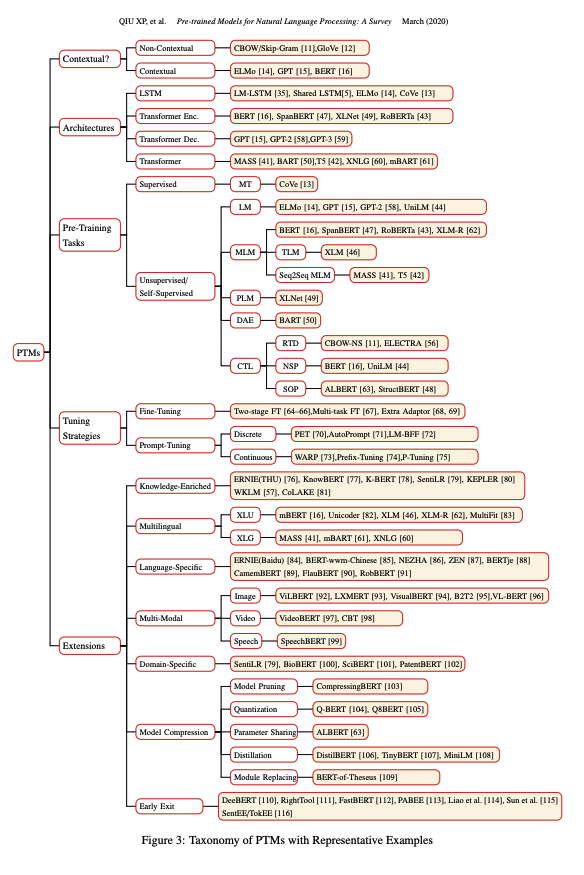
\includegraphics[width=\textwidth,height=\textheight,keepaspectratio]{02-08.png}
    \caption{Transformer taxonomy from \cite{qiu2020pre}}
    \label{fig:taxonomy}
\end{figure}


\bibliographystyle{unsrt}  
\bibliography{references}  %%% Remove comment to use the external .bib file (using bibtex).
%%% and comment out the ``thebibliography'' section.





\end{document}
